\documentclass[aoas,preprint, 11pt, dvipsnames, table, x11name]{imsart}

% natbib citation styles, see the natbib documentation, a copy of which
\usepackage{tikz-cd}
\usepackage[toc,page]{appendix}
\usepackage[font={small}, labelfont=bf]{caption}
\usepackage{subcaption}
\usepackage[utf8]{inputenc}
\newcommand{\E}{\mbox{E}}
\newcommand{\N}{\mbox{N}}
\graphicspath{{./figures/}}
\usepackage{amsfonts}
%Font
\usepackage[T1]{fontenc}
\usepackage{comment}
%\usepackage[dvipsnames,table,x11names]{xcolor}
\usepackage{xcolor}
\definecolor{darkgreen}{RGB}{0,69,0} %for rf
\definecolor{navy}{RGB}{0,60,113} %tough choice
\usepackage{booktabs}
\usepackage{bbm}
\usepackage{array}
\newcolumntype{P}[1]{>{\centering\arraybackslash}p{#1}}
\newcolumntype{P}[1]{>{\centering\arraybackslash}p{#1}}

\setlength{\parskip}{\baselineskip}
\usepackage{imakeidx}
\usepackage{tikz}
\usetikzlibrary{arrows.meta, calc, positioning}
%\usetikzlibrary{arrows}
\usetikzlibrary{positioning}
\newdimen\nodeDist{}
\nodeDist=25mm
\usepackage{pgfplots}
\newcommand{\indep}{\rotatebox[origin=c]{90}{$\models$}}
%\usepackage[english]{babel}
\usepackage{graphicx}
\usepackage{amsmath,commath,amssymb,blkarray,bm,bbm}
\usepackage{bbm}
\usepackage{mathtools}
\newcommand{\imp}[1]{\textbf{#1}}
\renewcommand{\bm}[1]{\mathbf{#1}}
\usepackage{mathrsfs}
\usepackage{physics}
\usepackage[pagebackref]{hyperref}  
\usepackage{comment}
\usepackage[authoryear]{natbib}
\bibliographystyle{plainnat}
\newcommand\independent{\protect\mathpalette{\protect\independenT}{\perp}}
\def\independenT#1#2{\mathrel{\rlap{$#1#2$}\mkern2mu{#1#2}}}
\DeclareMathOperator{\NA}{NA}
\newcommand{\ind}[1]{\mathbbm{1}({#1})}%
\hypersetup{
	colorlinks=true,
	linkcolor={blue},
	filecolor=magenta,      
	urlcolor={blue},
	citecolor={blue}
}
\bibliographystyle{imsart-nameyear}
\urlstyle{same}
%% Packages
\RequirePackage{amsthm,amsmath,amsfonts,amssymb}
\RequirePackage[authoryear]{natbib}
%\RequirePackage[colorlinks,citecolor=blue,urlcolor=blue]{hyperref}
%\RequirePackage{graphicx}

\startlocaldefs
%%%%%%%%%%%%%%%%%%%%%%%%%%%%%%%%%%%%%%%%%%%%%%
%%                                          %%
%% Uncomment next line to change            %%
%% the type of equation numbering           %%
%%                                          %%
%%%%%%%%%%%%%%%%%%%%%%%%%%%%%%%%%%%%%%%%%%%%%%
%\numberwithin{equation}{section}
%%%%%%%%%%%%%%%%%%%%%%%%%%%%%%%%%%%%%%%%%%%%%%
%%                                          %%
%% For Axiom, Claim, Corollary, Hypothezis, %%
%% Lemma, Theorem, Proposition              %%
%% use \theoremstyle{plain}                 %%
%%                                          %%
%%%%%%%%%%%%%%%%%%%%%%%%%%%%%%%%%%%%%%%%%%%%%%
%\theoremstyle{plain}
\newtheorem{axiom}{Axiom}
\newtheorem{claim}[axiom]{Claim}
\newtheorem{theorem}{Theorem}[section]
\newtheorem{lemma}[theorem]{Lemma}
%%%%%%%%%%%%%%%%%%%%%%%%%%%%%%%%%%%%%%%%%%%%%%
%%                                          %%
%% For Assumption, Definition, Example,     %%
%% Notation, Property, Remark, Fact         %%
%% use \theoremstyle{remark}                %%
%%                                          %%
%%%%%%%%%%%%%%%%%%%%%%%%%%%%%%%%%%%%%%%%%%%%%%
\theoremstyle{remark}
\newtheorem{definition}[theorem]{Definition}
\newtheorem*{example}{Example}
\newtheorem*{fact}{Fact}
%%%%%%%%%%%%%%%%%%%%%%%%%%%%%%%%%%%%%%%%%%%%%%
%% Please put your definitions here:        %%
%%%%%%%%%%%%%%%%%%%%%%%%%%%%%%%%%%%%%%%%%%%%%%

\endlocaldefs


\begin{document}
	\section{Estimating the risk difference as estimand of interest}\label{4.4}
	Rather than looking at the ratio of potential outcomes, it is often the case we want to investigate the difference in the expected value of each, i.e. we can look at \emph{risk differences}:
	\[\text{Risk Difference}\rightarrow \Delta \equiv \E(B^1)-E(B^0)\]
	In our framework, following similar reasoning as in section \emph{Modular sensitivity analysis with machine learning} in the main file,  risk differences can be defined as 
	\[\Delta(\mathbf{x}_i)=\int_{\mathbb{R}} \Phi\qty(b_1(\mathbf{x})+u)f(u)\dd u - \int_{\mathbb{R}} \Phi\qty(b_0(\mathbf{x})+u) f(u)\dd u\]
	The sample average risk difference (ARD) is therefore $\frac{1}{n}\sum_{i=1}^{n}\Delta(\mathbf{x}_i)$. In the case of the audit data, the average risk difference refers to percentage point difference in going bankrupt after receiving a going concern. We esimate the risk difference using our methodology as well as the bivariate probit with endogenous regressor model, (described in equation(4) in the main file), to the audit data.  Specifically, we used the same covariates as we used when fitting monotone bart, used the bankruptcy indicator as the binary outcome, and whether or not a going concern was issued as the ``treatment'' indicator.  Using our methodology, results for estimating risk differences on the audit data are presented in  \autoref{resultssummary}.
	
	
	\begin{table}[ht]
		\centering
		%	\scalebox{.9}{
		\begin{tabular}{lllllP{1.5cm}}
			\toprule
			$\gamma$&$\rho$& ARD true & ARD est&IRD cor&IRD RMSE \\ 
			\midrule
			1.00&0.25& 0.29 & 0.29 & 0.89 & 0.05  \\ 
			1.75&0.25& 0.47 & 0.47 & 0.96&0.04  \\ 
			2.50&0.25& 0.58 & 0.57 &  0.97&0.05  \\ 
			1.00&0.40 &0.29 & 0.29 &  0.90&0.05  \\ 
			1.75&0.40& 0.47 & 0.46 &  0.94&0.06  \\ 
			2.50&0.40& 0.58 & 0.55 &  0.96&0.09  \\ 
			1.00&0.60&  0.29 & 0.29 &  0.90&0.05  \\ 
			1.75&0.60& 0.47 & 0.46 &  0.95 &0.05 \\ 
			2.50&0.60& 0.58 & 0.57 & 0.98&0.04  \\ 
			1.00&0.80& 0.29 & 0.27 &  0.91&0.05  \\ 
			1.75&0.80& 0.47 & 0.44 &  0.95 &0.05 \\ 
			2.50&0.80 &0.58 & 0.55 &  0.98&0.05 \\
			\bottomrule
		\end{tabular}
		%}
		
		\caption{We simulate from the bivariate probit with 25,000 observations and deploy our methodology.  cor refers to the correlation between predicted and true for the average risk difference (ARD), and the rmse is the root mean square error. Fit using the `GJRM' package of \cite{marra}.}
		\label{bivartable_treat}
	\end{table}
	
%	When fitting the bivariate probit regression, parameters are estimated using maximum likelihood. Our ARD from this regression was 2.90 percentage points and a mean risk ratio of 2.82 with 95\% CI (1.33, 6.04).  Note, we used a regression spline approach to smooth our numeric covariates, where the smooth term for each covariate is made of basis functions, see \cite{marra} for details.  This gives us additional flexibility in fitting the model.
	
	\begin{table}[t]
		\centering
		%	\begin{bclogo}[couleur=newblue!74!white, arrondi=0.16, logo=\bcplume ,, ombre=true, barre=none ]{}
		%\begin{tabular}{lllll}%{P{1.6cm}P{1.5cm}P{1.5cm}P{1.5cm}P{1.5cm}P{2cm}}
		\begin{tabular}{lP{1.1cm}P{1.1cm}P{1.1cm}P{2.9cm}}
			%	\toprule
			%	&\color{BrickRed}\textbf{XGBoost}&\color{darkgreen}\textbf{Random Forest}&\color{navy}\textbf{BART}\\ \midrule
			%\multicolumn{2}{c}Method&\multicolumn{2}{c}{\color{BrickRed}{XGBoost}} &\multicolumn{2}{c}{\color{darkgreen}{Random %Forest}}&\multicolumn{2}{c}{\color{navy}{BART}}\\
			%	\midrule
			\toprule
			Distribution of $f(u)$  & ARD (\%)&ARD post (\%)& mean $B_1$ (\%) &95\% Credible interval for ARD (\%)  \\ \midrule
			$\N(0,\sigma=0.1)$ &9.92&9.97&11.5&$\qty(7.08, 12.9)$\\ %\hline
			$\N(0,\sigma=0.5)$ &3.95&4.12 &5.96 &$\qty(2.74, 5.60)$\\%\hline      
			$\N(0,\sigma=1)$&0.45&0.70&2.90&$\qty(0.40, 1.01)$\\
			Shark $q=0.25$, $s=0.5$; $\sigma=1.05$&0.12&0.28&2.60&$\qty(0.14, 0.45)$\\
			Shark $q=0.75$, $s=1.25$; $\sigma=0.89$&2.62&2.84&4.87&$\qty(1.81, 3.97)$\\
		%	98\% peak $\sigma=0.29$&6.85&7.08&8.62&$\qty(5.41, 9.06)$\\
			90\% peak $\sigma=0.64$&2.04&2.30&4.52&$\qty(2.23, 2.92)$\\
					
			Asymmetric Mixture $\sigma=0.49$&2.20&2.47&4.62&$\qty(2.43, 3.14)$\\
			%	80\% peak&1.66&4.30&100\\
			
			\bottomrule%\\\midrule %\hline       
			%total&333&435&66&47&& \\ \bottomrule        
		\end{tabular}
		%\captionsetup{labelformat=empty}
		\caption{The reduced form probabilities (equation (15) in the main file) were estimated using BART with a monotonicity constraint on the going concern variable.  We further require $b_1(\bm{x})>b_0(\bm{x})$ in the projection step.  Posterior summaries based on 500 Monte Carlo samples.  $\sigma$ refers to the implied standard deviations of the different distributions.  Values listed as the percentage increase in probability of bankruptcy.}
		%\caption{LHS of system of equations \ref{long} estimated using BART with monotonicity constraint.  Additional constraint in optimization/integration step requires $b_1(\bm{x})>b_0(\bm{x})$.  Credible interval based on quantiles of random sample of 500 posterior draws.  Interpret the inducement as percentage point increase in probability of bankruptcy.  $\sigma$ in the shark fin refers to implied standard deviation given $q$ and $s$ parameters. The mean $\tau$ column refers to the mean inducement effect calculated by solving the integral formulation of \ref{maineq} once with LHS probabilities given by the mean of the BART posterior estimate. mean $\tau$ post refers to the mean of the inducement effect after solving the system of equations for each 500 posterior draws of the estimates of the LHS probabilities of \ref{maineq}, and mean $B_1$ refers to the mean bankruptcy probability (including the treatment effect).}
		\label{resultssummary}
		%\end{bclogo}
	\end{table}
	
	
	It was stressed in the main document how using  BART with a monotonicity constraint improves our estimation of the ICRR, but the improvement is even more pronounced when studying risk differences.  
	In figure \autoref{monovsnorm_ITE}, we look at the comparison of IRD (individual risk difference) estimates from data generated by the bivariate probit, with the left hand side of our system of equation probabilites estimated with BART and monotone BART.  We display in the main file, but with inducements as the estimand of interest.
	\begin{figure}[t]
		\centering
		\begin{subfigure}{.5\textwidth}
			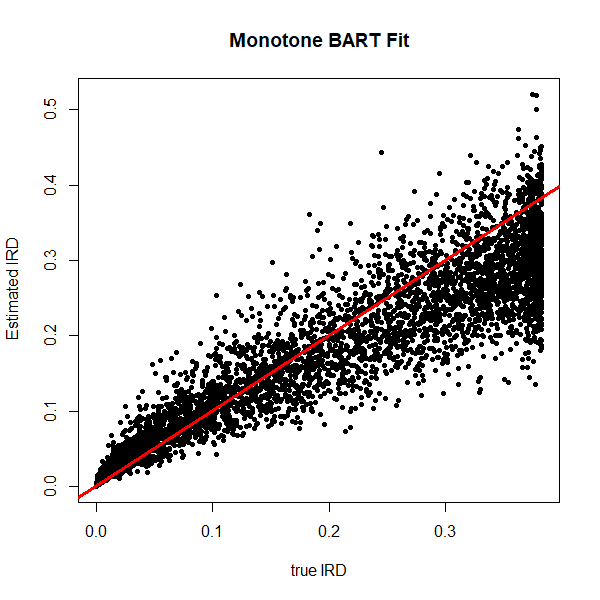
\includegraphics[width=6.cm]{monobartITE_png.png}
		\end{subfigure}%
		\begin{subfigure}{.5\textwidth}
			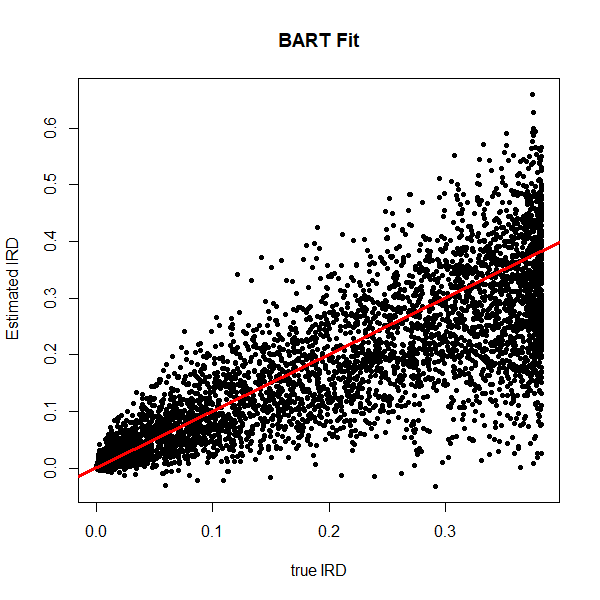
\includegraphics[width=6.cm]{BartITE_png.png}
		\end{subfigure}
		\caption{Plots of expected individual risk differences (IRD) vs our estimates, i.e. a plot comparing the difference in potential outcomes from the bivariate probit model ($\Phi(\alpha_0+\alpha_1\bm{x}_i+\gamma)-\Phi(\alpha_0+\alpha_1\bm{x}_i)$) versus our estimate.  In the DGP, $\rho=0.25,\gamma=1$.  The monotone BART correlation between $\tau$ and $\hat{\tau}$ is 0.928 and for BART is 0.826}
		\label{monovsnorm_ITE}
	\end{figure}
	
	\section{Bivariate probit simulation study}\label{bivar_append}
	 \autoref{bivarvalidate} shows the results when fitting the bivariate probit regression with a maximum likelihood estimate to the simulated bivariate probit data.  Unsurprisingly, this performs well, with the caveat that we require large $\N$ ($\N=100,000$) to get these impressive results.  We simulated the samples from the bivariate probit model of the main document, where we sum 5 uniform(-1,1) $\bm{x}_i$ covariates each with the same $\beta_1$ and $\alpha_1$ coefficients respectively.  We set $\beta_0=0, \beta_1=-0.2, \alpha_0=-0.5, \alpha_1=0.7$ to generate reasonable number of going concerns and bankruptcies.
	
	 \autoref{bivartable_treat} shows the results when we simulate from the bivariate probit and fit with our methodology, with $f(u)$ assigned appropriately, only this time we are interested in the treatment effect.  Our method does well here, with $\N=25,000$ and $p=5$.  
	
	\begin{table}[t]
		\centering
		\scalebox{.85}{
			\begin{tabular}{lllP{1.3cm}P{1.3cm}P{1.3cm}P{1.3cm}P{1.3cm}llll}
				\toprule
				ARD true & ARD est&IRD cor&IRD RMSE&ACRR true&ACRR est& ICRR cor&ICRR rmse&  $\gamma$ true&$\gamma$ est.& $\rho$& $\rho$ est. \\ 
				\midrule
				0.23 & 0.24 & 0.97 & 0.02 & 2.24 & 2.07 & 1.00 & 0.24 & 1.00 & 0.77 & 0.25 & 0.37 \\ 
				0.46 & 0.46 & 0.99 & 0.02 & 4.32 & 3.89 & 1.00 & 0.87 & 1.75 & 1.62 & 0.25 & 0.31 \\ 
				0.58 & 0.57 & 1.00 & 0.02 & 6.24 & 5.40 & 0.99 & 2.34 & 2.50 & 2.38 & 0.25 & 0.30 \\ 
				0.26 & 0.26 & 0.99 & 0.01 & 2.42 & 2.27 & 1.00 & 0.22 & 1.00 & 0.85 & 0.40 & 0.47 \\ 
				0.46 & 0.46 & 0.99 & 0.02 & 4.33 & 3.89 & 1.00 & 0.90 & 1.75 & 1.63 & 0.40 & 0.45 \\ 
				0.57 & 0.56 & 0.99 & 0.02 & 6.14 & 5.13 & 1.00 & 2.83 & 2.50 & 2.34 & 0.40 & 0.46 \\ 
				0.28 & 0.28 & 0.99 & 0.01 & 2.57 & 2.46 & 1.00 & 0.17 & 1.00 & 0.92 & 0.60 & 0.63 \\ 
				0.47 & 0.47 & 1.00 & 0.01 & 4.51 & 4.24 & 1.00 & 0.63 & 1.75 & 1.70 & 0.60 & 0.61 \\ 
				0.59 & 0.58 & 1.00 & 0.01 & 6.41 & 5.89 & 0.99 & 1.67 & 2.50 & 2.45 & 0.60 & 0.61 \\ 
				0.31 & 0.31 & 1.00 & 0.00 & 2.79 & 2.80 & 1.00 & 0.02 & 1.00 & 1.02 & 0.80 & 0.80 \\ 
				0.47 & 0.47 & 1.00 & 0.01 & 4.51 & 4.26 & 1.00 & 0.56 & 1.75 & 1.70 & 0.80 & 0.81 \\ 
				0.58 & 0.58 & 1.00 & 0.01 & 6.31 & 5.56 & 0.99 & 2.25 & 2.50 & 2.41 & 0.80 & 0.82 \\ 
				\bottomrule
			\end{tabular}
		}
		\caption[Bivariate probit regression validation]{N=100,000. Fit the simulated bivariate probit with the bivariate probit regression.  Validates the MLE of the bivariate probit regression performs well, as well as the validity of our data generation process, however required a large $N$ to get accurate results. ARD refers to average risk difference, IRD individual risk difference.  ACRR refers to average causal risk ratio, whereas ICRR is individual causal risk ratio. }
		\label{bivarvalidate}
	\end{table}

	\newpage
	\section{Comparing machine learning methods for the observational data}\label{machine_append}
	Here we present our results from fitting the left hand side of equation(15) in the main file.
	In this section, we compare the performance in predicting the left hand side of equation(15) using various non-parametric ``machine learning'' tools.  In particular, we compare using monotone BART \footnote{We use a BART \citep{bart} model for the $\Pr(G\mid \bm{x})$ scenario, consistent with the main text.}, random forests \citep{rf}, and xgboost \citep{boost}. Referencing \autoref{roc_plot} seems to indicate our methodology outperforms competitors in a cross-validation assessment.\footnote{In our main text, we do not do a cross validation to obtain our probabilities, but rather get the probabilities from deploying the monotone BART models on the entire dataset.  In this case, our $B_1,G_0$ auc was 0.88, $B_1, G_1$ was 0.83, and $G_1$ was 0.92.}. 
	
	%These differences manifest themselves on the right side of table \ref{roc_table}, where the estimates of the inducement effect vary depending on method. 
	
	%Because monotone BART looks to be the best performer and because of the added benefit of monotonicity constraint, we continue our analysis using the BART estimates from here on out. 
	
	
	
	
	
	\begin{figure}[t]
		
		\begin{minipage}[t]{.5\textwidth}
			
			
			%	\centering
			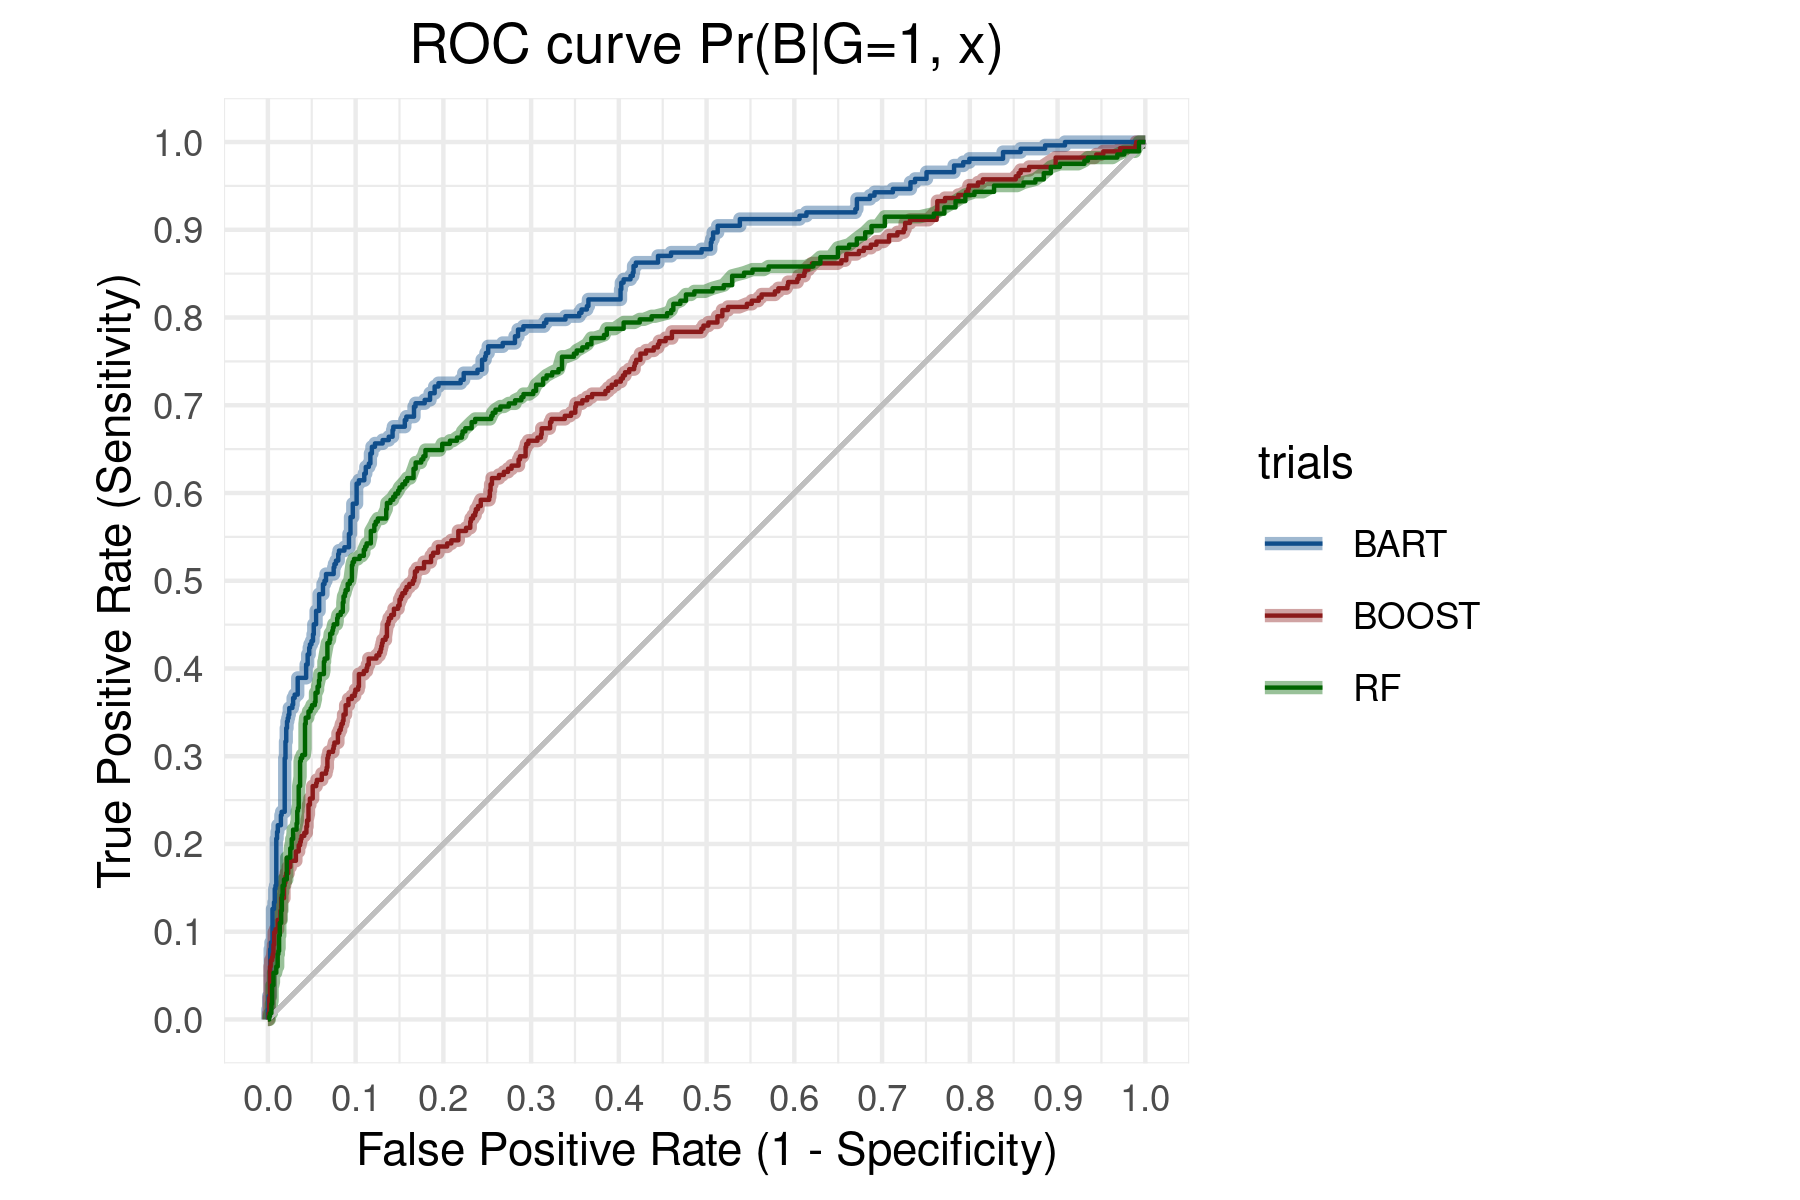
\includegraphics[width=8cm]{roc_pbg1_cv_png}
			
			
			
		\end{minipage}\hfill
		\begin{minipage}[t][-2.2cm][b]{.5\textwidth}	
			\centering
			%\begin{tabular}{lllll}%{P{1.6cm}P{1.5cm}P{1.5cm}P{1.5cm}P{1.5cm}P{2cm}}
			\begin{tabular}{P{1.1cm}P{1.2cm}P{1.25cm}P{1.25cm}}
				%	\toprule
				&\color{BrickRed}\textbf{XGBoost}&\color{darkgreen}\textbf{RanFor}&\color{navy}\textbf{BART}\\ \midrule
				%\multicolumn{2}{c}Method&\multicolumn{2}{c}{\color{BrickRed}{XGBoost}} &\multicolumn{2}{c}{\color{darkgreen}{Random %Forest}}&\multicolumn{2}{c}{\color{navy}{BART}}\\
				%	\midrule
				
				Case   & AUC  & AUC & AUC  \\ \midrule
				$B_1, G_0$ &0.80&0.83&0.87\\ %\hline
				\rowcolor{navy!49!white}$B_1, G_1$ &0.73 &0.78&0.83 \\%\hline      
				$G_1$ &0.88&0.90&0.90 \\ \bottomrule%\\\midrule %\hline       
				%total&333&435&66&47&& \\ \bottomrule        
			\end{tabular}
			
			
		\end{minipage}
		\caption{Left: Area under curve of ROC plot, balanced 5-fold CV.  Plot of ROC performance for predicting $\Pr(B\mid G=1, \bm{x})$ .  Corresponds to shaded row in table on right.  Right:  case 1 is predicting bankruptcy when no going concern is issued, case 2 is when no concern issued, and case 3 predicts if concern is issued.  All the methods are \emph{similar}, with monotone BART seeming to be the top performer.}
		\label{roc_plot}
	\end{figure}
	\begin{comment}
	%	\caption{Classification correct percentage.  Notice that the situation matters but in general BART appears to be the most accurate.  Case 1 is predicting bankruptcy when no going concern is issued, which explains why all methods were more accurate, as firms rarely go bankrupt without showing reason for concern in the prior year.}
	%	\label{resultstable}
	\end{subtable}%
	\begin{subtable}{.5\textwidth}
	\centering
	\begin{tabular}{P{.4cm}P{.7cm}P{.6cm}P{.8cm}P{.7cm}P{.7cm}P{.4cm}}%{lllllll}%{P{1.6cm}P{1.5cm}P{1.5cm}P{1.5cm}P{1.5cm}P{2cm}}
	%toprule??
	%\toprule  
	%	\toprule
	%	\multicolumn{1}{c}{}&\multicolumn{2}{c}{\color{BrickRed}\textbf{XGBoost }} &\multicolumn{2}{c}{\color{darkgreen}\textbf{Ran-For}}&\multicolumn{2}{c}{\color{navy}\textbf{BART}}\\
	%	\midrule
	
	&	\color{BrickRed}\textbf{XGBoost}&&\color{darkgreen}\textbf{RanFor}&&\color{navy}\textbf{BART}&\\ \midrule
	$\sigma$ &$\mu(\tau)$ &$\mu(B_1$) &$\mu(\tau)$  & $\mu(B_1)$&$\mu(\tau)$   &$\mu(B_1)$  \\ \midrule
	$0.1$ &7.63&9.17&10.6&11.9&8.89&10.3\\ %\hline
	$0.5$ &3.56 &5.27&4.51 &5.91&3.62&5.29 \\%\hline      
	$1$ &0.86&2.91&1.22&2.90&0.41&2.57 \\ \bottomrule %\hline       
	%	total&333&435&66&47&& \\ \bottomrule             
	\end{tabular}
	
	\end{subtable}
	\caption{Left: Area under curve of ROC plot, balanced 5-fold CV.  Case 1 is predicting bankruptcy when no going concern is issued, case 2 is when no concern issued, and case 3 predicts if concern is issued. Right:Results when fitting to the different $\sigma$ for the mean 0 Gaussian curves.  $\mu(\tau)$ is the average inducement effect in percentage point increase.  $\mu(B_1)$ is the mean of bankrupftcy given going concern potential outcome.  }
	\label{roc_table}
	\end{table}
	\end{table}
	\begin{figure}[h]
	\centering
	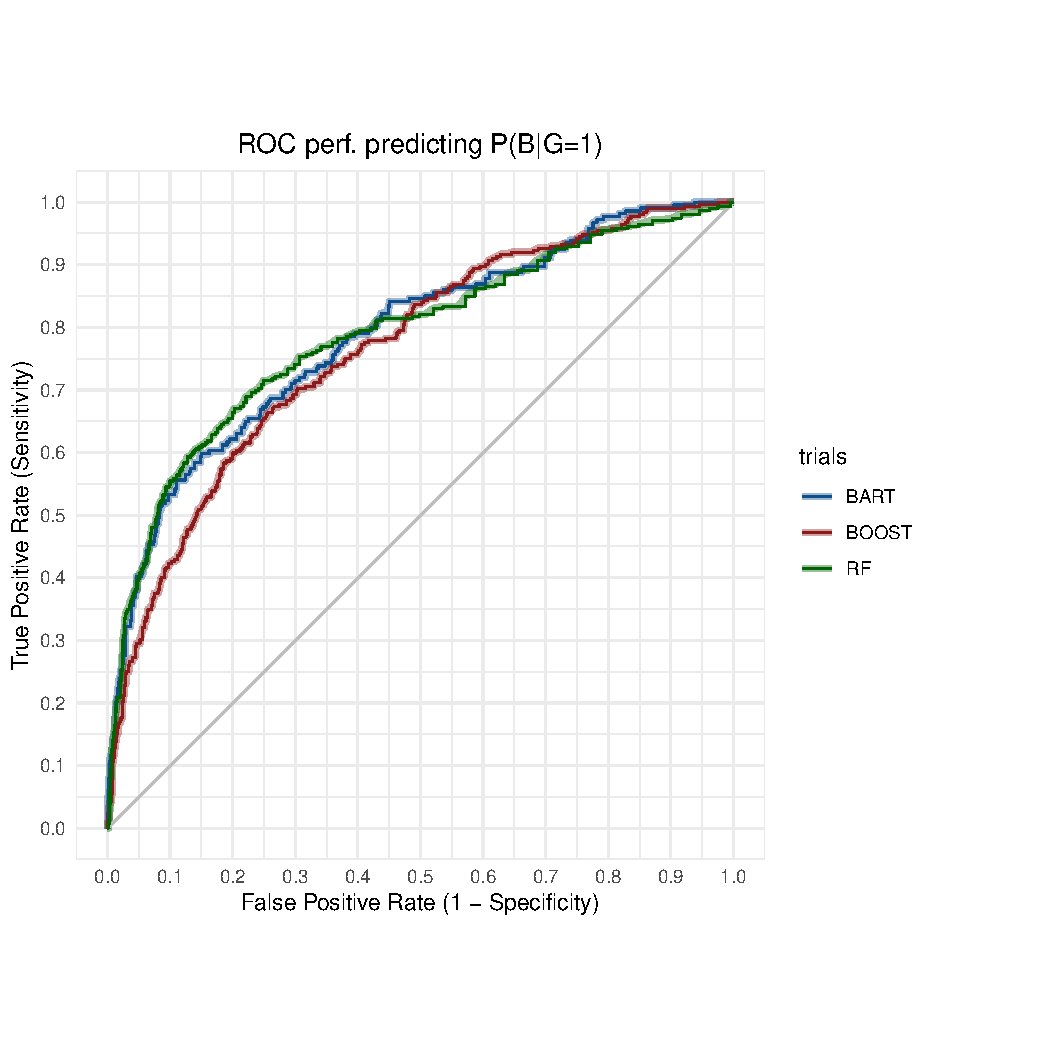
\includegraphics[width=8cm]{roc_pbg1_cv}
	\caption{Plot of ROC performance. Here is the case where we predict probability of bankruptcy given a going concern.  Corresponds to shaded row in table \ref{roc_table}.  All the methods are \emph{similar}, with monotone BART seeming to be the top performer.}
	\label{roc_plot}
	\end{figure}
	\clearpage
	\section{Average treatment effect as the estimand of interest}\label{ATE_append}
	In this section, we explore the average treatment effect (ATE) as the estimand of interest.  The ATE is a commonly studied estimand, but we relegate much of the discussion to the appendix to emphasize the comparison between our methodology and the E-value, which is reported on the risk-ratio scale.  
	In figure \ref{monovsnorm_ITE}, we look at the comparison of ITE estimates from data generated by the bivariate probit, with the left hand side of our system of equation probabilites estimated with BART and monotone BART.  This is a similar plot to \ref{monovsnorm}, but with a different estimand of interest.
	\begin{figure}[h]
	\centering
	\begin{subfigure}{.5\textwidth}
	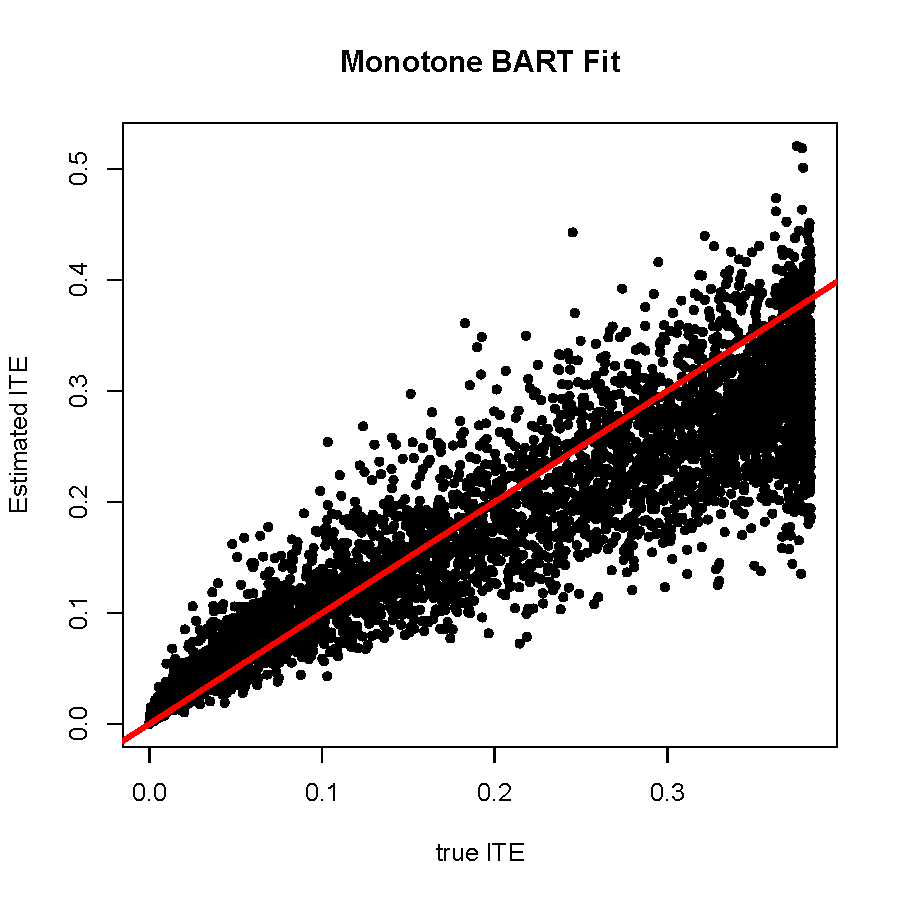
\includegraphics[width=7.cm]{monobartITE.pdf}
	\end{subfigure}%
	\begin{subfigure}{.5\textwidth}
	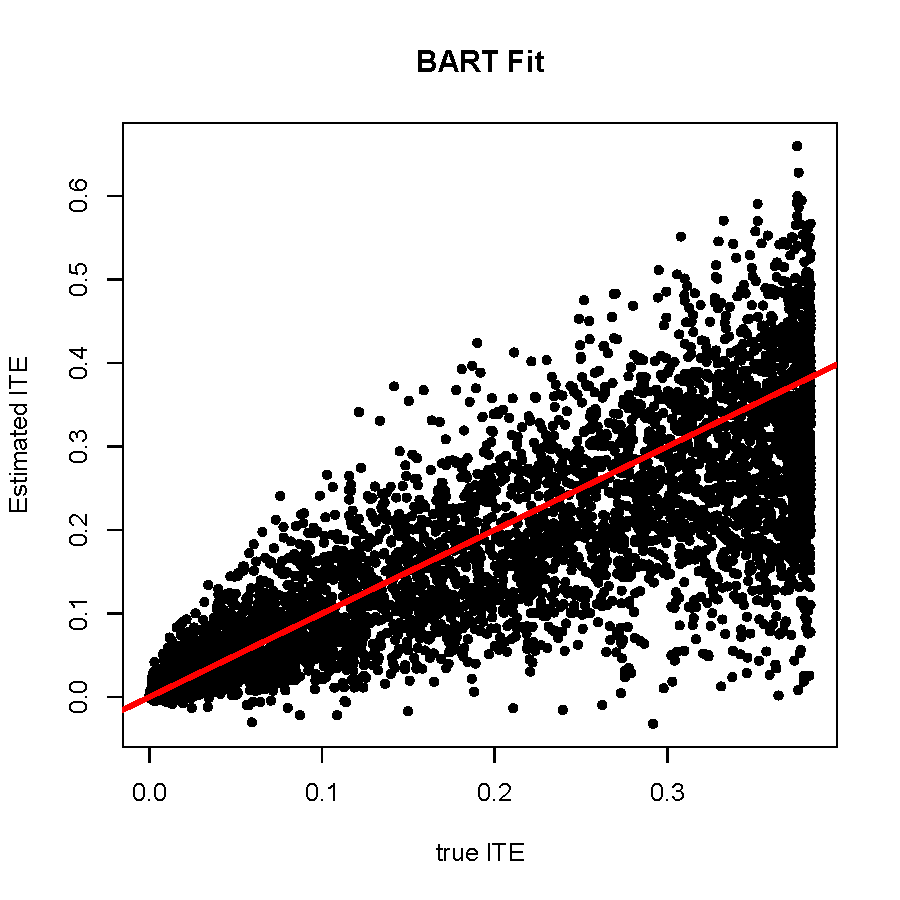
\includegraphics[width=7.cm]{BartITE.pdf}
	\end{subfigure}
	\caption{Plots of expected individual treatment effects vs our estimates, i.e. a plot comparing the difference in potential outcomes from model \ref{latentutility} ($\Phi(\alpha_0+\alpha_1\bm{x}_i+\gamma)-\Phi(\alpha_0+\alpha_1\bm{x}_i)$) versus our estimate within the integral of equation(\ref{treateq}).  In the DGP, $\rho=0.25,\gamma=1$.  The monotone BART correlation between $\tau$ and $\hat{\tau}$ is 0.928 and for BART is 0.826}
	\label{monovsnorm_ITE}
	\end{figure}
	\begin{comment}
	\begin{figure}[h]
	\centering
	\begin{subfigure}{.5\textwidth}
	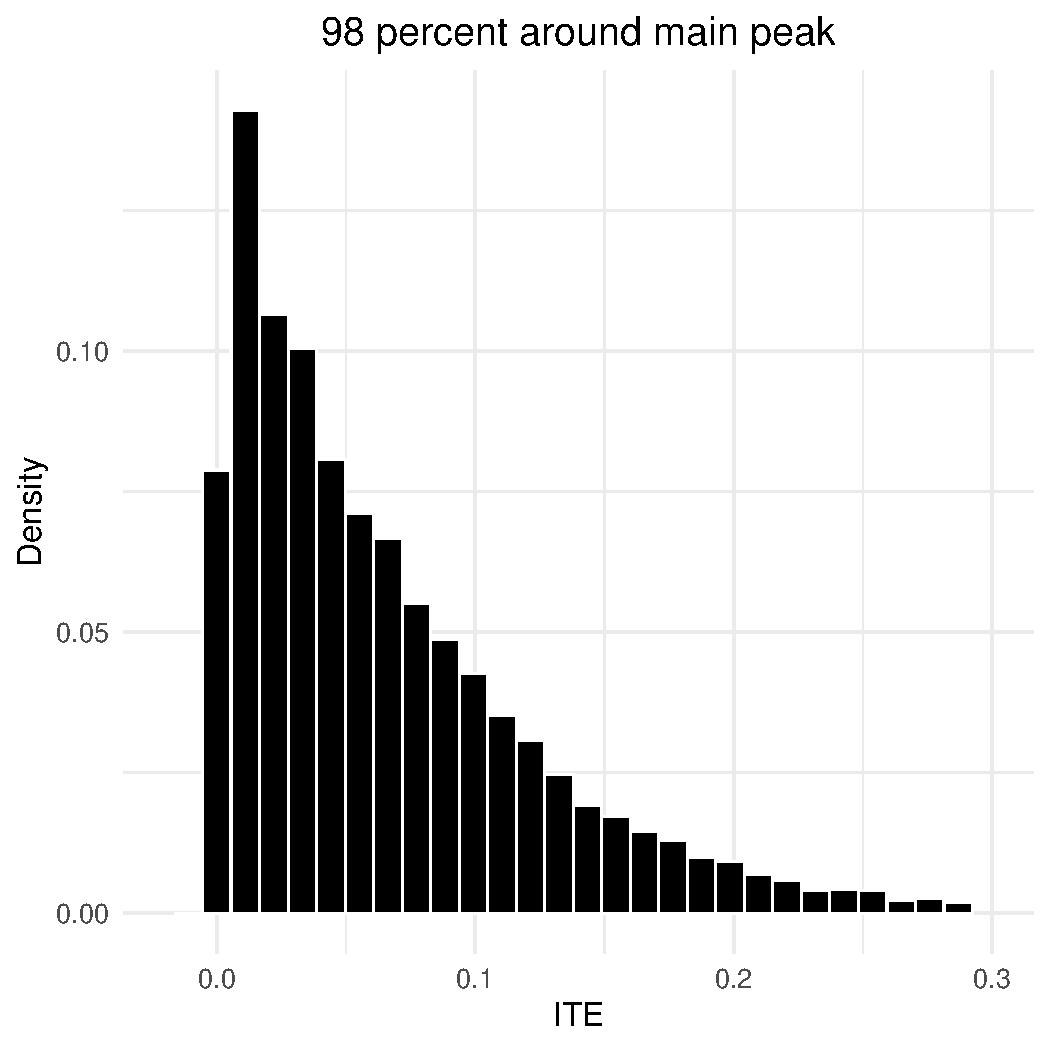
\includegraphics[width=7cm]{symmetric1percbump_constrained.pdf}
	\end{subfigure}%
	\begin{subfigure}{.5\textwidth}
	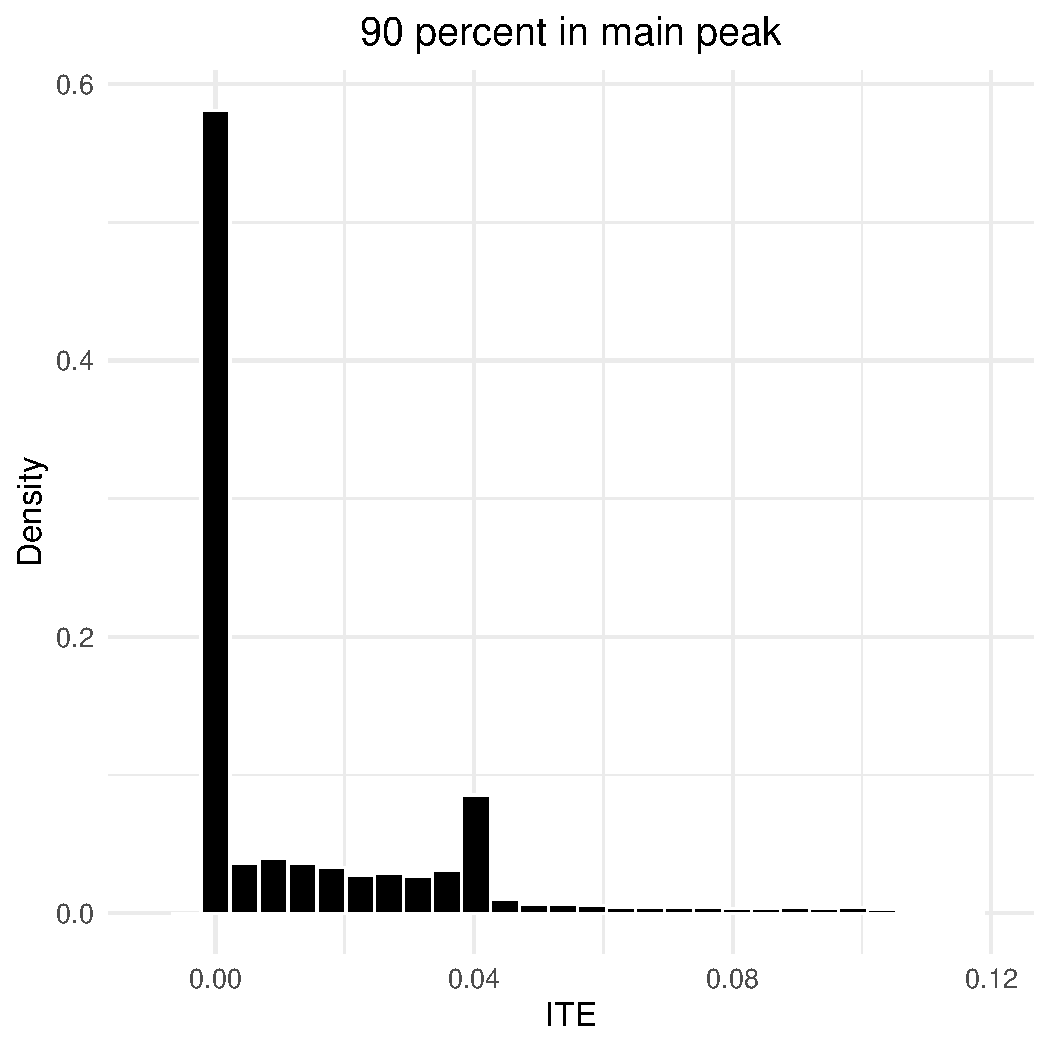
\includegraphics[width=7cm]{symmetric5percbump_constrained.pdf}
	\end{subfigure}
	%	\begin{subfigure}{.3\textwidth}
	%		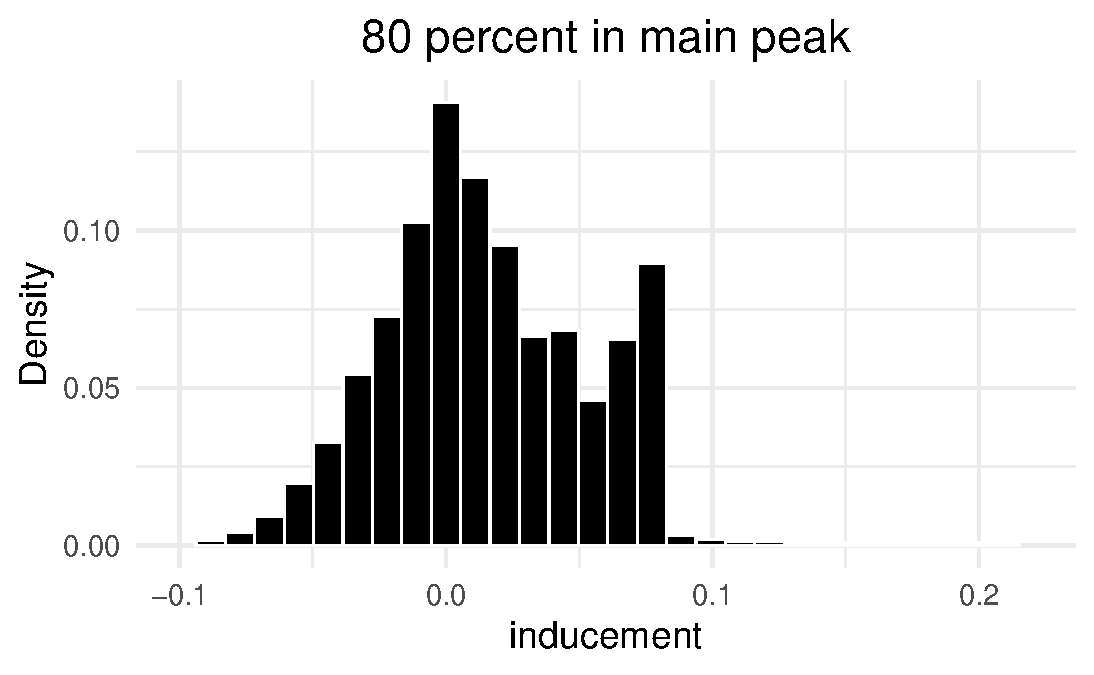
\includegraphics[height=5.3cm, width=4.8cm]{symmetric10percbump}
	%	\end{subfigure}
	\caption{Histogram of individual treatment effects across all the firms in our dataset.  The distributions of $u$ respectively are Gaussian mixtures and have 98\% and 90\% of their weight centered around 0 with $\sigma=0.05$, with the rest centered evenly around -2 and 2 respectively, again with $\sigma=0.05$.  See table \ref{resultssummary} for summary of average inducement effect estimates.}%The means for inducement are 0.071, 0.015, and 0.017. Interpret as 7.1$\%$, 1.5\%, and 1.7\%.  Notice that with even 10 percent of the data centered around a mean $u$ of 2 and -2, there is very little inducement effect, indicating $u=2$ is a large 2.  Means of $B_1$ are 8.08\%, 3.80\%, and 4.30\%.}
	\label{multiresults}
	\end{figure}
	
	\begin{figure}[h]
	\centering
	\begin{minipage}{.5\textwidth}
	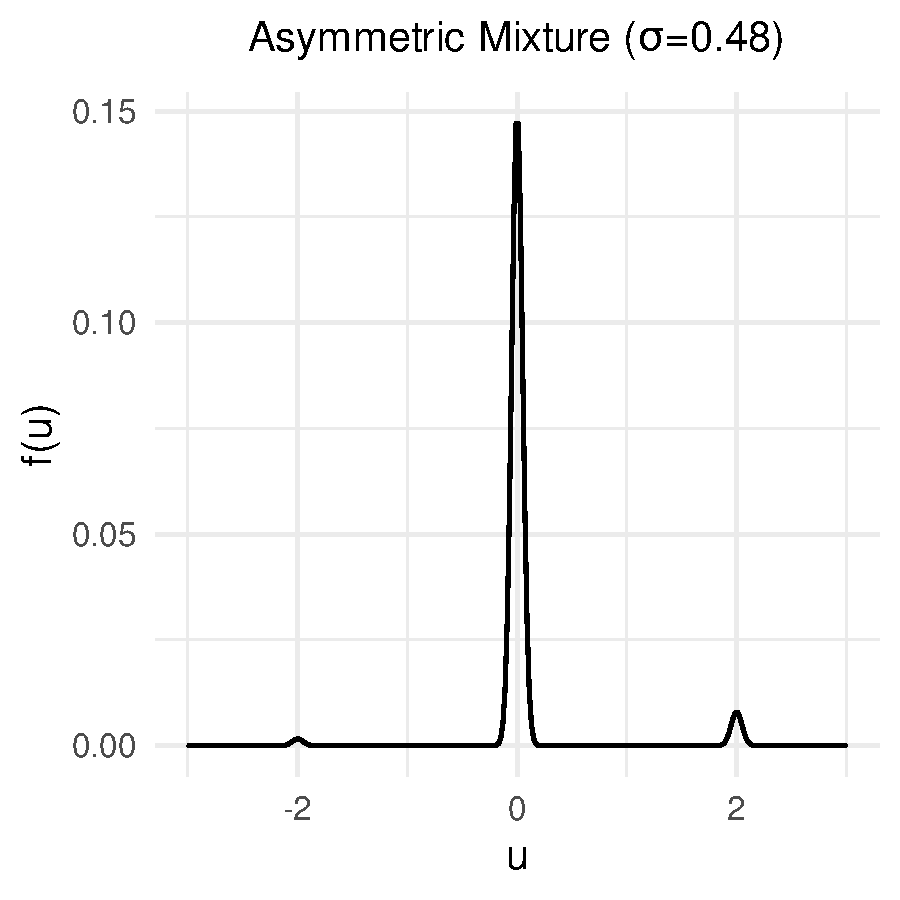
\includegraphics[width=6cm]{rightbump2}
	\end{minipage}%
	\begin{minipage}{.5\textwidth}
	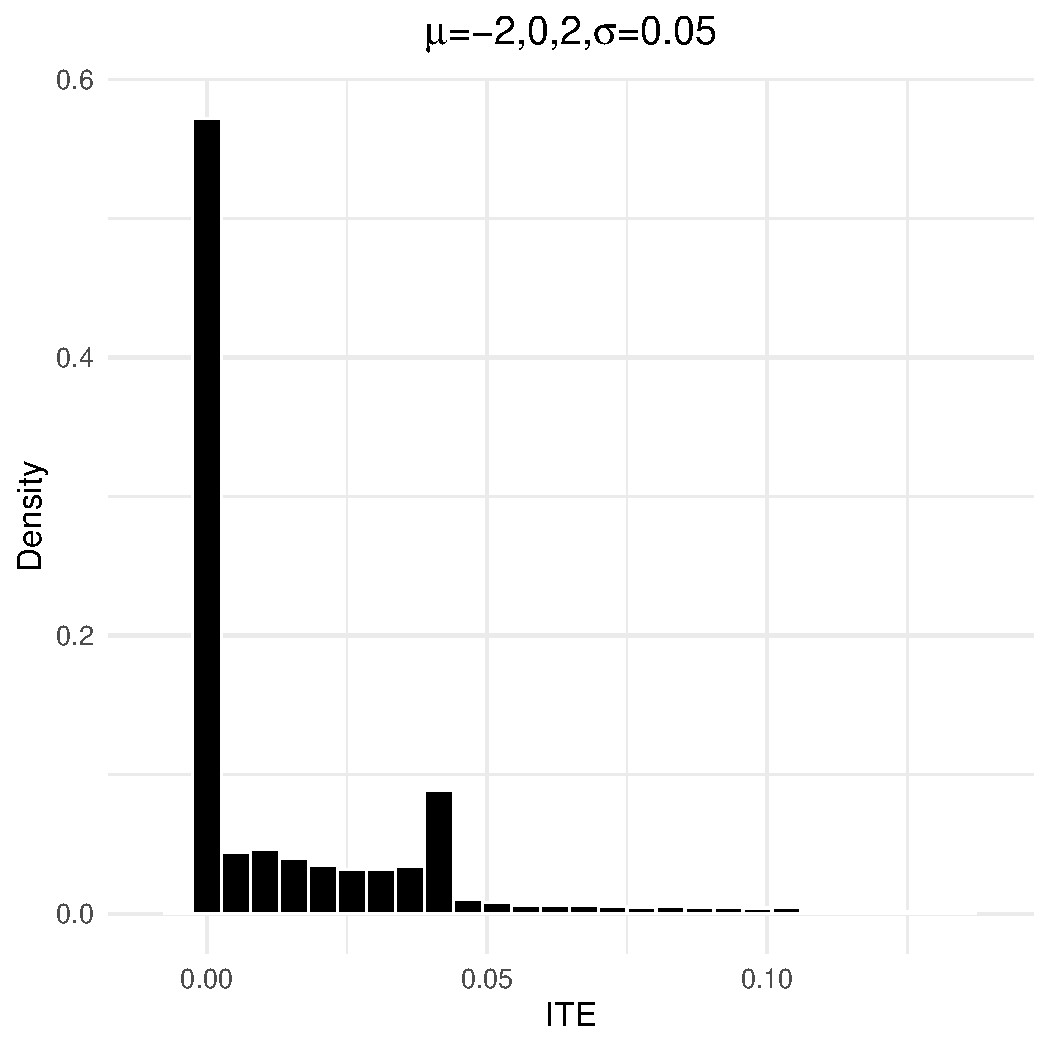
\includegraphics[width=6cm]{gammarightmore2_constrained.pdf}
	\end{minipage}
	\caption{$f(u)$ was specified according to the figure on the left. 94\% of the mass is centered around 0, 1\% around -2, and 5\% around 2, indicating the hidden information is more likely to lead to  probability of bankruptcy to approach 1 than 0.  The mean for inducement is a 1.68\% point increase in the probability of bankruptcy, and the mean probability of bankrupcty is 3.87\%.}
	\label{rightbump}
	\end{figure}
	
	
	\begin{table}[h]
	\centering
	%	\begin{bclogo}[couleur=newblue!74!white, arrondi=0.16, logo=\bcplume ,, ombre=true, barre=none ]{}
	%\begin{tabular}{lllll}%{P{1.6cm}P{1.5cm}P{1.5cm}P{1.5cm}P{1.5cm}P{2cm}}
	\begin{tabular}{lP{1.1cm}P{1.1cm}P{1.1cm}P{1.5cm}P{2.3cm}}
	%	\toprule
	%	&\color{BrickRed}\textbf{XGBoost}&\color{darkgreen}\textbf{Random Forest}&\color{navy}\textbf{BART}\\ \midrule
	%\multicolumn{2}{c}Method&\multicolumn{2}{c}{\color{BrickRed}{XGBoost}} &\multicolumn{2}{c}{\color{darkgreen}{Random %Forest}}&\multicolumn{2}{c}{\color{navy}{BART}}\\
	%	\midrule
	\toprule
	Distribution of $f(u)$  & ATE (\%)&ATE post& mean $B_1$ (\%)&mean $\frac{B_1}{B_0}$ &95\% Credible interval for ATE (\%)  \\ \midrule
	$N(0,\sigma=0.1)$ &8.89&8.91&10.3&29.2&$\qty(6.95, 11.2)$\\ %\hline
	$N(0,\sigma=0.5)$ &3.62&3.76 &5.29&9.32 &$\qty(2.78, 4.97)$\\%\hline      
	$N(0,\sigma=1)$&0.41&0.63&2.57&1.56&$\qty(0.37, 0.97)$\\
	Shark q=0.25, $\sigma=0.5$; var=1.11&0.11&0.24&2.44&1.08&$\qty(0.13, 0.40)$\\
	Shark q=0.75, $\sigma=1.25$; var=0.77&2.39&2.57&4.30&7.53&$\qty(1.82, 3.52)$\\
	
	``Right Bump'' $\sigma=0.05$&1.98&2.17&4.10&5.21&$\qty(1.78, 2.69)$\\
	98\% peak&6.85&7.08&8.62&24.6&$\qty(5.41, 9.06)$\\
	90\% peak&1.85&2.03&4.02&4.98&$\qty(1.68, 2.51)$\\
	%	80\% peak&1.66&4.30&100\\
	
	\bottomrule%\\\midrule %\hline       
	%total&333&435&66&47&& \\ \bottomrule        
	\end{tabular}
	%\captionsetup{labelformat=empty}
	\caption{LHS of system of equations \ref{long} estimated using BART with monotonicity constraint.  Additional constraint in optimization/integration step requires $b_1(\bm{x})>b_0(\bm{x})$.  Credible interval based on quantiles of random sample of 500 posterior draws.  Interpret the inducement as percentage point increase in probability of bankruptcy.  var in the shark fin refers to implied variance given $q$ and $\sigma$ parameters. The mean $\tau$ column refers to the mean inducement effect calculated by solving the integral formulation of \ref{maineq} once with LHS probabilities given by the mean of the BART posterior estimate. mean $\tau$ post refers to the mean of the inducement effect after solving the system of equations for each 500 posterior draws of the estimates of the LHS probabilities of \ref{maineq}, and mean $B_1$ refers to the mean bankruptcy probability (including the treatment effect).}
	\label{resultssummary}
	%\end{bclogo}
	\end{table}
	
	\end{comment}
	
	
	
	
	
	
	
	\begin{comment}
	Presented in table \ref{table_compare} is a comparison between select sensitivity analysis estimates of the ATE and the estimate from the bivariate probit regression.
	
	
	\begin{table}[h]
	\centering
	%	\begin{bclogo}[couleur=newblue!74!white, arrondi=0.16, logo=\bcplume ,, ombre=true, barre=none ]{}
	%\begin{tabular}{lllll}%{P{1.6cm}P{1.5cm}P{1.5cm}P{1.5cm}P{1.5cm}P{2cm}}
	\begin{tabular}{lll}%{P{4.9cm}P{3.1cm}}
	%	\toprule
	%	&\color{BrickRed}\textbf{XGBoost}&\color{darkgreen}\textbf{Random Forest}&\color{navy}\textbf{BART}\\ \midrule
	%\multicolumn{2}{c}Method&\multicolumn{2}{c}{\color{BrickRed}{XGBoost}} &\multicolumn{2}{c}{\color{darkgreen}{Random %Forest}}&\multicolumn{2}{c}{\color{navy}{BART}}\\
	%	\midrule
	\toprule
	Run   & ATE (\%)   \\ \midrule
	$N(0,0.5)$ &3.62  \\%\hline      
	$N(0,1)$&0.41 \\
	%	``Right Bump'' $\sigma=0.02$&8.07\\
	%\rowcolor{navy!49!white}
	``Right Bump'' $\sigma=0.05$&1.98\\
	98\% peak&6.85\\
	90\% peak&1.85\\
	
	%80\% peak&4.3\\
	%	Full ID $\gamma$ vary&0.08\\
	%	Full ID $\gamma$ constant over firms&3.79\\ %\\\midrule %\hline   
	Bivariate Probit Regression& 2.90\\  
	\bottomrule%\\\midrule %\hline       
	%total&333&435&66&47&& \\ \bottomrule        
	\end{tabular}
	%\captionsetup{labelformat=empty}
	\caption{Comparison of the average treatment effect using different methods.}
	\label{table_compare}
	%\end{bclogo}
	\end{table}
	
	\end{comment}
	
	% \begin{table}[h]
	% 	\centering
	% 	\begin{tabular}{P{2cm}P{2cm}P{2cm}P{2cm}P{2cm}}
	% 		\toprule
	% 		$\tau$ est. & $\tau$ true &  $\gamma$ & $\rho$& $\rho$ est. \\ 
	% 		\midrule
	% 		0.204 & 0.201 & 1 & 0.25 & 0.246 \\ 
	% 		0.384&0.396&2&0.25&0.196\\
	% 		0.507&0.507&3&0.25&0.238\\
	% 		0.571&0.575&4&0.25&0.209\\
	% 		0.596&0.599&5&0.25&0.205\\
	% 		0.204&0.195&1&0.40&0.416\\
	% 		0.384&0.392&2&0.40&0.366\\
	% 		0.507&0.505&3&0.40&0.397\\
	% 		0.571&0.571&4&0.40&0.384\\
	% 		0.596&0.594&5&0.40&0.390\\
	% 		0.204&0.195&1&0.6&0.616\\
	% 		0.384&0.390&2&0.60&0.582\\
	% 		0.507&0.503&3&0.60&0.605\\
	% 		0.571&0.567&4&0.60&0.607\\
	% 		0.596&0.591&5&0.60&0.605\\
	% 		0.204&0.195&1&0.80&0.811\\
	% 		0.384&0.383&2&0.80&0.800\\
	% 		0.507&0.499&3&0.80&0.811\\
	% 		0.571&0.568&4&0.80&0.799\\
	% 		0.596&0.591&5&0.80&0.802\\
	% 		0.143&0.130&0.7&0.60&0.625\\
	% 		\bottomrule
	% 	\end{tabular}
	% 	\caption{N=100000. Validates the MLE of the bivariate probit regression performs well, as well as the validity of our data generation process.   }
	% 	\label{bivarvalidate}
	% \end{table}
	\begin{comment}
	\section*{Appendix B.}
	
	One form of verification would be to use experimental data to confirm our method works in the case of no unobserved confounding.  
	The experiment of interest is one ran by Salagnik and Watts, known as ``Success and Failure in Cultural Markets'' \citep{music}.  In their experiment, the authors tested the whether or not the popularity of a song causes a song to become more popular.  The researchers deployed two different experiments with varying levels of ``influence'' as the treatment. In the first experiment, users in the treatment group see how often their peers downloaded a song, whereas users in the control group were shown the songs without knowing how many times others users in the experiment downloaded the song.  In experiment 2, the strong influence experiment, users in the treatment group were shown how many times each song was downloaded by other users in the treatment, and the songs with the most downloads were placed at the top of the screen.  The control group was set-up similarly.  This experiment mirrors the situation with the auditors, with the social influence and song download playing the roles of the going concern and bankruptcy.
	
	
	The data provided with the experiment included information about the users who partook in the experiment.  From the features of the users, we were able to predict probabilities of song download in both the treatment world (the influence condition) and the control world.  Because our data come from an experiment, presumably the users are randomly assigned to the control/treatment worlds.  Due to the control group being bigger than each of the treatment groups of each repetition of either experiment, both the Bart and Random Forest methods were over-fitting the  
	propensity score.  To remedy this, we randomly sampled the control world to match the sample size of the treatment world.  
	
	In figure \ref{graph2}, we present histograms of the treatment effects, calculated from equation (\ref{treateq}) across individuals in the weak and strong social influence experiments for each of the 8 repetitions of the experiment.   These are the situations where we used Bart to predict the joint probabilities in the left hand side of equation(\ref{long}). For our distribution of $U$, we assigned $U\sim N(0,0.1)$ to simulate the conditions where unobserved confounding plays a minimal role.  
	
	
	We appear to do a good job in returning the correct ATE.  The percentile (0-1 scale) of the actual ATE compared to the distribution of treatment effect is denoted by \% actual in figure\ref{graph2}.  Table \ref{tabl1} also shows our method is returning essentially unbiased estimates of the ATE, meaning our method seems to be well verified in the case of no unobserved confounding.  This gives more faith in the ability of tree-based methods, particularly BART, to accurately predict bankruptcy and going-concern probabilities.
	
	
	\begin{table}[h]
	\centering
	\begin{tabular}{rrr}
	\toprule
	World& $\sigma=0.1$ ATE  & actual ATE \\ 
	\midrule
	1 & 0.165 & 0.168 \\ 
	2 & 0.165  & 0.166 \\ 
	3 & 0.131 & 0.133 \\ 
	4 & 0.170  & 0.175 \\ 
	5 & 0.180  & 0.179 \\ 
	6 & 0.134 & 0.136 \\ 
	7 & 0.158  & 0.166 \\ 
	8 & 0.180  & 0.183 \\ 
	\bottomrule
	\end{tabular}
	\caption{Experiment 2.  We compare our estimated ATE calculated from equation (\ref{treateq}) and fitting predicted probabilities to the actual ATE calculated directly from the data.}
	\label{tabl1}
	\end{table}
	
	
	\begin{figure}[h]
	\centering
	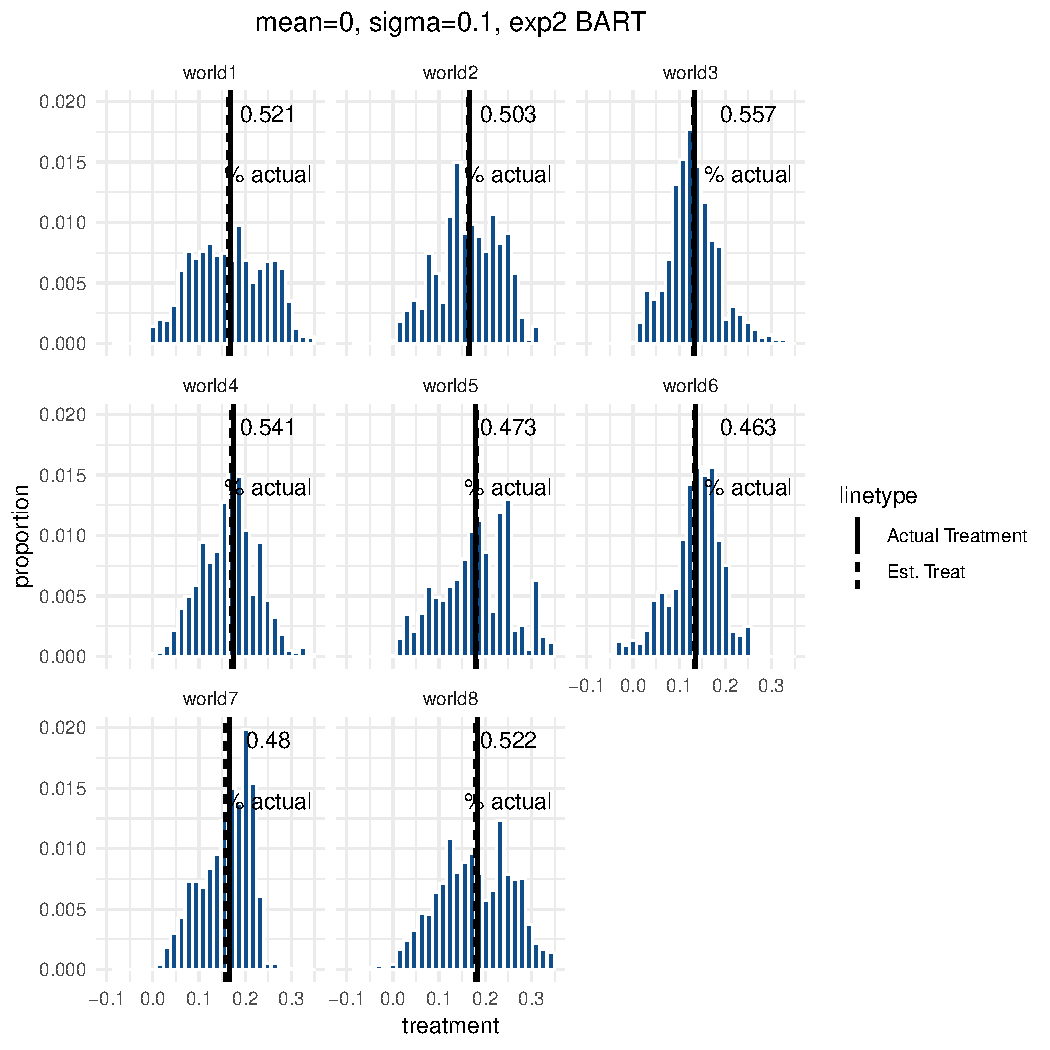
\includegraphics[height=12cm, width=15cm]{exp2graph1bart.pdf}
	
	\caption{Histogram of treatment effect by user for experiment 2, the strong influence case.  Probabilities fit using BART.  The distribution of $U$ is $N(0,0.1)$, essentially representing a case with no unobserved confounding.}
	\label{graph2}
	\end{figure}
	\end{comment}
	
	\begin{comment}
	\subsection{Exploratory subgroup analysis}\label{4.5}
	We follow similar methodology to that proposed in \cite{bcffreak}.  We identifty moderating subgroup of variables by fitting a single regression tree which regresses the ITE estimates on the moderating covariates.  Our set of moderating covariates is the same as the covariates presented in \ref{4.1}, as all of those variables (or groups of them) could potentially serve as moderators.  
	
	We fit the regression tree to the ITE estimates provided from running monotone BART with $f(u)\sim N(0, \sigma=0.5)$.  We choose the subgroup with the largest ATE, as in figure \ref{cart_tree}.  For the 70 firms in this subgroup, we again estimate the left hand side of equation(\ref{maineq}), except now keep all 2000 posterior draws from BART. Previously, in the audit data and in simulations, we estimated the LHS of equation(\ref{maineq}) by taking the mean of the posterior draws from BART. We then solve our integral equations for these 70 firms for each of the 2000 posterior draws, and then averaging across all the firms for each draw gives us a fully Bayesian posterior summary of the ATE for this subgroup.  This was repeated for 4 different distributions of $f(u)$, see figure \ref{mod_plot}.  The 4 distributions are: $f_1(u)\sim N(0,\sigma=.5)$, $f_2\sim N(0,1)$, $f_3(u)$  is a a mixture model with more weight on a far bump to the right, see figure \ref{individ_firm_plot}, and $f_4(u)$ is a 3 component Gaussian mixture with 90\% of the area centered around 0, and 5\% around $u=-2$ and $u=2$ respectively.
	\begin{figure}[ht]
	\centering
	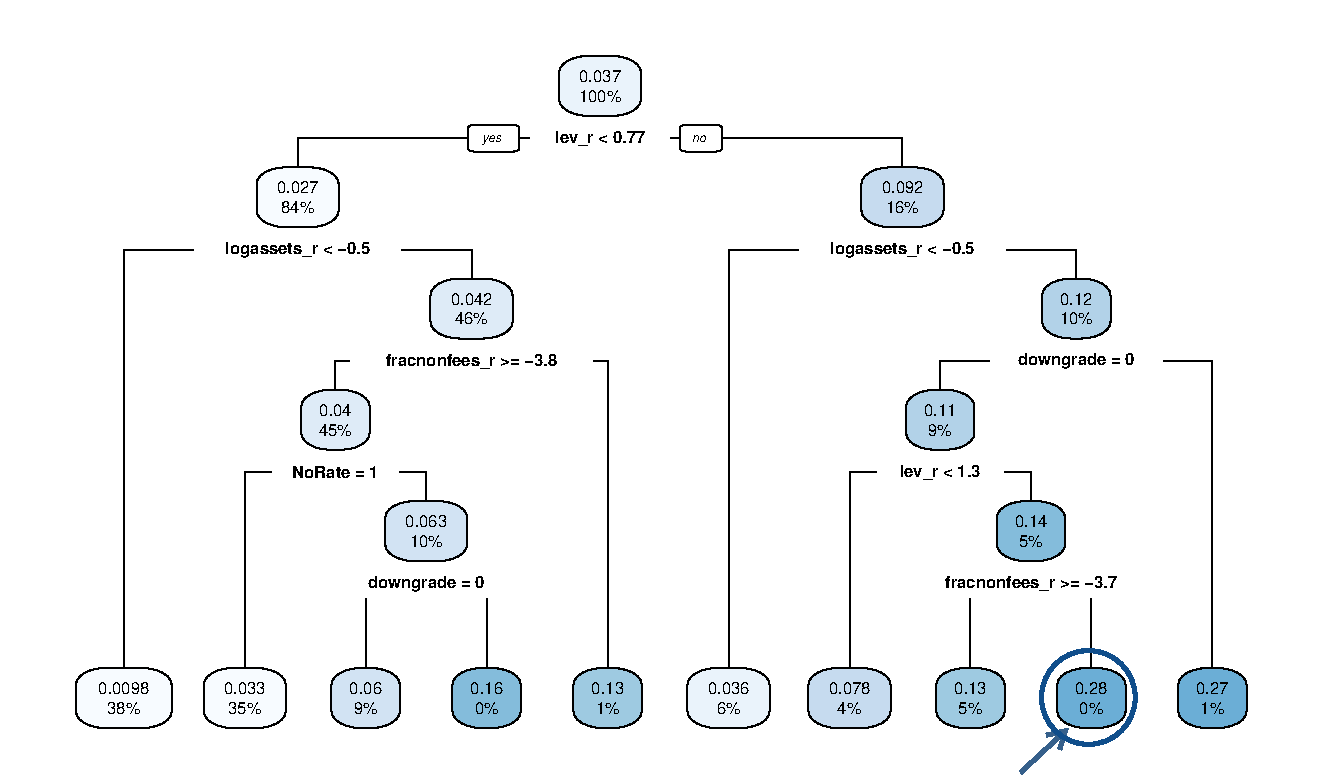
\includegraphics[ width=12cm]{cart_tree}
	\caption{The second box from the bottom right is the subgroup of interest, which signifies the largest subgroup ATE.  This is also the group of variables we investigate as moderators, seen in figure \ref{mod_plot}. Follow down tree to identify subgroup.}%	\caption{ The arrow points to the subgroup of interest, which signifies the largest subgroup ATE.  This is also the group of variables we investigate as moderators, seen in figure \ref{mod_plot}. Follow down tree to identify subgroup.}
	\label{cart_tree}
	\end{figure}
	
	
	
	
	\begin{figure}[ht]
	\centering
	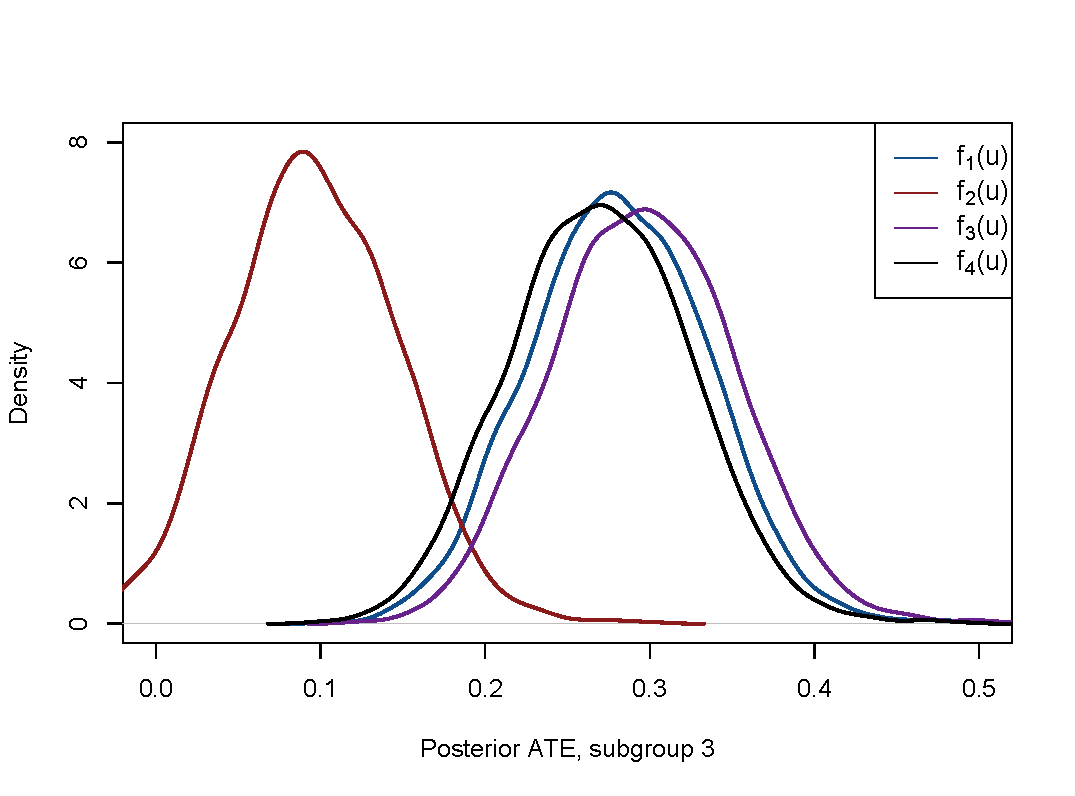
\includegraphics[ width=10cm]{ATE_subgroup3}
	\caption{Plot of posterior density ATE subgroup 3. The mean ATE estimates across the 2000 posterior draws for the 4 different $f(u)$ are 0.28, 0.10, 0.30, 0.27 respectively. }
	\label{mod_plot}
	\end{figure}
	\end{comment}
	\color{black}
	
	
	\begin{comment}
	\begin{table}[h]
	\centering
	%		\begin{bclogo}[couleur=newblue!74!white, arrondi=0.16, logo=\bcplume ,, ombre=true, barre=none ]{}
	%\begin{tabular}{lllll}%{P{1.6cm}P{1.5cm}P{1.5cm}P{1.5cm}P{1.5cm}P{2cm}}
	\begin{tabular}{lP{1.5cm}P{1.5cm}P{1.5cm}P{1.5cm}P{2.9cm}}
	%	\toprule
	%	&\color{BrickRed}\textbf{XGBoost}&\color{darkgreen}\textbf{Random Forest}&\color{navy}\textbf{BART}\\ \midrule
	%\multicolumn{2}{c}Method&\multicolumn{2}{c}{\color{BrickRed}{XGBoost}} &\multicolumn{2}{c}{\color{darkgreen}{Random %Forest}}&\multicolumn{2}{c}{\color{navy}{BART}}\\
	%	\midrule
	\toprule
	Firm   &Going Concern&Bankruptcy& Auditor&mean $\tau$ post &95\% Credible interval for $\tau$ (\%)  \\ \midrule
	Jetblue (2007)&No&No&E\&Y&5.69&$(0.71, 14.2)$\\
	%\rowcolor{navy!49!white}
	Jetblue (2009)&No&No&E\&Y&3.42&$(0.00, 10.5)$\\
	%\rowcolor{navy!49!white}
	Apple (2001) &No&No&KPMG&6.06&$(0.85, 17.6)$\\
	Build a Bear (2010)&No&No&KPMG&1.68&$(0.10, 4.60)$\\
	Build a Bear (2014)&No&No&E\&Y&3.58&$(0.81, 8.36)$\\
	Radioshack (2013)&No&No&PWC&17.6&$(0.41, 39.4)$\\
	Radioshack (2014)&No&Yes&PWC&10.8&$(0.00, 31.2)$\\
	Blockbuster (2004)&No&No&PWC&2.16&$(0.14, 6.67)$\\
	Blockbuster (2009)&Yes&No&PWC&13.9&$(1.73, 29.0)$\\
	Six Flags (2006)&No&No&KPMG&6.72&$(0.67, 16.4)$\\
	Six Flags (2009)&Yes&Yes&KPMG&16.4&$(0.72, 39.0)$\\
	\bottomrule       
	\end{tabular}
	%	\captionsetup{labelformat=empty}
	\caption[Different ATE estimates for specific firms]{Posterior estimates of the treatment effect given $f(u)\sim N(0, \sigma=0.5)$, here we look at the mean of the posterior estimates of the treatment effect for different firms in our dataset. }
	\label{individ_firm_table}
	%	\end{bclogo}
	\end{table}
	
	\begin{figure}[h]
	\centering
	\includegraphics[width=14cm]{Apple_jetblue_ITE}
	\caption[Apple vs Jetblue]{Histogram of posterior estimates of the individual treatment effects given $f(u)\sim N(0, \sigma=0.5)$ (moderate confounding) for Apple 2001 and Jetblue 2009.  Neither received a going concern, nor did either go bankrupt.  Jetblue was audited by Ernst and Young, and Apple audited by KPMG.} 
	\label{individ_firm_plot}
	\end{figure}
	\end{comment}
	
	\begin{comment}
	\begin{table}[!htb]
	\centering
	\begin{subtable}{.5\textwidth}
	
	%\begin{tabular}{lllll}%{P{1.6cm}P{1.5cm}P{1.5cm}P{1.5cm}P{1.5cm}P{2cm}}
	\begin{tabular}{lP{1.cm}P{.6cm}P{1.55cm}}
	\midrule
	%\multicolumn{2}{c}Method&\multicolumn{2}{c}{\color{BrickRed}{XGBoost}} &\multicolumn{2}{c}{\color{darkgreen}{Random %Forest}}&\multicolumn{2}{c}{\color{navy}{BART}}\\
	%	\midrule
	&\textbf{Subgroup3 ATE:0.28}&&\\ \midrule
	$\Pr(G\mid \bm{x})$ values&\#obs, \# bank&E-value&95\% CI E-Value  \\ \midrule
	$[8.7\mathrm{e}{-3}, 0.23]$&14, 3&5.45&$(\NA, 1.00)$\\
	$(0.23, 0.36]$&14, 4&5.85&$(\NA,1.00)$\\ 
	$(0.36, 0.51]$&14, 7&2.37&$(\NA,1.00)$\\
	$(0.53, 0.69]$&14, 8&4.78&$(\NA,1.00)$\\
	$(0.69, 0.86]$&14,12&NA&$(\NA,\NA)$\\
	\bottomrule%\\\midrule %\hline       
	%total&333&435&66&47&& \\ \bottomrule        
	\end{tabular}
	%	\caption{Subgroup 4, this is the subgroup in the farthest bottom right in figure \ref{cart_tree}.}
	
	
	\end{subtable}%
	\begin{subtable}{.5\textwidth}
	
	%\begin{tabular}{lllll}%{P{1.6cm}P{1.5cm}P{1.5cm}P{1.5cm}P{1.5cm}P{2cm}}
	\begin{tabular}{lP{1.cm}P{.6cm}P{1.55cm}}
	\midrule
	%\multicolumn{2}{c}Method&\multicolumn{2}{c}{\color{BrickRed}{XGBoost}} &\multicolumn{2}{c}{\color{darkgreen}{Random %Forest}}&\multicolumn{2}{c}{\color{navy}{BART}}\\
	%	\midrule
	&\textbf{Subgroup4 ATE:0.27}&&\\ \midrule
	$\Pr(G\mid \bm{x})$ values&\#obs, \# bank&E-value&95\% CI E-Value  \\ \midrule
	$[5.4\mathrm{e}{-3}, 0.16]$&35, 3&1.33&$(1.00, \NA)$\\
	$(0.16, 0.35]$&35, 8&3.97&$(\NA,1.00)$\\ 
	$(0.35, 0.53]$&35,14&4.10&$(\NA,1.00)$\\
	$(0.53, 0.71]$&34,18&7.72&$(\NA,2.14)$\\
	$(0.71, 0.92]$&34,21&12.4&$(\NA,1.00)$\\
	\bottomrule%\\\midrule %\hline       
	%total&333&435&66&47&& \\ \bottomrule        
	\end{tabular}
	%	\caption{Subgroup 4, this is the subgroup in the farthest bottom right in figure \ref{cart_tree}.}
	
	
	\end{subtable}
	\caption[E-value calculations for subgroups]{Top left: Subgroup 1, this is the subgroup in the farthest bottom left in figure \ref{cart_tree}. Top right: Subgroup 2, this is the subgroup in the second from farthest bottom left in figure \ref{cart_tree}. Bottom left: Subgroup 3, this is the subgroup in the  second from farthest bottom right in figure \ref{cart_tree}. Bottom right: Subgroup 4, this is the subgroup in the farthest bottom right in figure \ref{cart_tree}.}
	\end{table}
	
	\end{comment}
	\begin{comment}
	We additionally calculate E-values for various subgroups identified in figure \ref{cart_tree}.  We choose two subgroups that had small effects and two with the largest effects.  
	
	\begin{table}[h]
	\centering
	%\begin{bclogo}[couleur=newblue!74!white, arrondi=0.16, logo=\bcplume ,, ombre=true, barre=none ]{}
	%\begin{tabular}{lllll}%{P{1.6cm}P{1.5cm}P{1.5cm}P{1.5cm}P{1.5cm}P{2cm}}
	\begin{tabular}{P{3.4cm}P{3.1cm}P{2.1cm}P{2.5cm}}%P{3.1cm}}
	%	\toprule
	%	&\color{BrickRed}\textbf{XGBoost}&\color{darkgreen}\textbf{Random Forest}&\color{navy}\textbf{BART}\\ \midrule
	%\multicolumn{2}{c}Method&\multicolumn{2}{c}{\color{BrickRed}{XGBoost}} &\multicolumn{2}{c}{\color{darkgreen}{Random %Forest}}&\multicolumn{2}{c}{\color{navy}{BART}}\\
	%	\midrule
	\toprule
	$\Pr(G\mid \bm{x})$ values& \# obs, \# bankruptcy&Evalue&95\% CI\\ \midrule % Median $P(G\mid \bm{x})$& Evalue\\ \midrule
	$[0, .19]$& 20896,228&16.03&(11.7, NA)\\ %0.16&16.03\\%8.08\\
	$(0.19, 0.37]$&2456,135&7.86&(5.45, NA)\\%0.258%7.86\\%2.50\\
	$(0.37, 0.55]$&1204,100&6.86&(4.11, NA)\\%0.45&6.86\\%1.22\\
	$(0.55, 0.74]$&630,78&5.15&(2.60, NA)\\%0.620&5.15\\%1.87\\
	$(0.74, 0.92]$&164,37&13.0&(1.00, NA)\\ %0.783&13.04\\%3.59\\ 		
	
	\bottomrule%\\\midrule %\hline       
	%total&333&435&66&47&& \\ \bottomrule        
	\end{tabular}
	%\captionsetup{labelformat=empty}
	\caption{$\Pr(G\mid \bm{x})$ are propensity score estimates from monotone BART.  We split the propensity score into 5 bins, then for each bin calculate the risk ratio by comparing bankruptcies of the binned data with the going concern being issued in each bin according to the dataset. The overall averaged E-value across all bins is 14.52, indicating it is likely that the inducement effect is indeed causal, though the E-value varies greatly for different estimates of the propensity score. }
	\label{evaluetable}
	%\end{bclogo}
	\end{table}
	
	\begin{table}[!htb]
	\centering
	%\begin{tabular}{lllll}%{P{1.6cm}P{1.5cm}P{1.5cm}P{1.5cm}P{1.5cm}P{2cm}}
	\begin{subtable}{.5\textwidth}
	
	%\begin{tabular}{lllll}%{P{1.6cm}P{1.5cm}P{1.5cm}P{1.5cm}P{1.5cm}P{2cm}}
	\begin{tabular}{P{1.25cm}P{1.25cm}P{.8cm}P{2.05cm}}
	\midrule
	%\multicolumn{2}{c}Method&\multicolumn{2}{c}{\color{BrickRed}{XGBoost}} &\multicolumn{2}{c}{\color{darkgreen}{Random %Forest}}&\multicolumn{2}{c}{\color{navy}{BART}}\\
	%	\midrule
	&\textbf{Subgroup1 ATE:0.001}&&\\ \midrule
	$\Pr(G\mid \bm{x})$ values&\# obs, \# bank&E-value&95\% CI E-Value  \\ \midrule
	$[0, 0.18]$&7202,38&9.85&(4.23, NA)\\
	$(0.18, 0.36]$&1530,44&3.34&(1.40,NA)\\ 
	$(0.36, 0.54]$&672,27&1.47&(1.00,NA)\\
	$(0.54, 0.7267,9&3.61&(1.00,NA)\\1]$&
	$(0.71, 0.89]$&48,2&$\NA$&(NA, NA)\\
	\bottomrule%\\\midrule %\hline       
	%total&333&435&66&47&& \\ \bottomrule        
	\end{tabular}
	%	\caption{Subgroup 1, this is the subgroup in the farthest bottom left in figure \ref{cart_tree}.}
	
	
	\end{subtable}%
	\begin{subtable}{.5\textwidth}
	
	%\begin{tabular}{lllll}%{P{1.6cm}P{1.5cm}P{1.5cm}P{1.5cm}P{1.5cm}P{2cm}}
	\begin{tabular}{P{1.25cm}P{1.25cm}P{.8cm}P{2.05cm}}
	\midrule
	%\multicolumn{2}{c}Method&\multicolumn{2}{c}{\color{BrickRed}{XGBoost}} &\multicolumn{2}{c}{\color{darkgreen}{Random %Forest}}&\multicolumn{2}{c}{\color{navy}{BART}}\\
	%	\midrule
	&\textbf{Subgroup2:ATE 0.03}&&\\ \midrule
	$\Pr(G\mid \bm{x})$ values&\#obs, \# bank&E-value&95\% CI E-Value  \\ \midrule
	$[0, 0.12]$&8419,61&29.8&(16.0, NA)\\
	$(0.12, 0.24]$&375,10&23.99&(6.00,NA)\\ 
	$(0.24, 0.36]$&113,9&12.3&(2.13,NA)\\
	$(0.36, 0.48]$&41,2&$\NA$&(NA, $\NA$)\\
	$(0.48, 0.59]$&12,1&NA&(NA, $\NA$)\\
	\bottomrule%\\\midrule %\hline       
	%total&333&435&66&47&& \\ \bottomrule        
	\end{tabular}
	%	\caption{Subgroup 2, this is the subgroup in the second from farthest bottom left in figure \ref{cart_tree}.}
	
	
	\end{subtable}
	\end{table}
	\begin{table}[!htb]
	\centering
	\begin{subtable}{.5\textwidth}
	
	%\begin{tabular}{lllll}%{P{1.6cm}P{1.5cm}P{1.5cm}P{1.5cm}P{1.5cm}P{2cm}}
	\begin{tabular}{P{1.25cm}P{1.25cm}P{.8cm}P{2.05cm}}
	\midrule
	%\multicolumn{2}{c}Method&\multicolumn{2}{c}{\color{BrickRed}{XGBoost}} &\multicolumn{2}{c}{\color{darkgreen}{Random %Forest}}&\multicolumn{2}{c}{\color{navy}{BART}}\\
	%	\midrule
	&\textbf{Subgroup3 ATE:0.28}&&\\ \midrule
	$\Pr(G\mid \bm{x})$ values&\#obs, \# bank&E-value&95\% CI E-Value  \\ \midrule
	$[0.01, 0.18]$&10,10&NA&(NA,NA)\\
	$(0.18, 0.35]$&16,6&16.2&(1.82, NA)\\ 
	$(0.35, 0.52]$&15, 7&2.37&(1.00, NA)\\
	$(0.52, 0.69]$&15, 9&3.41&(1.00, NA)\\
	$(0.69, 0.86]$&13,11&1&(1.00,1.00)\\
	\bottomrule%\\\midrule %\hline       
	%total&333&435&66&47&& \\ \bottomrule        
	\end{tabular}
	%\caption{Subgroup 3, this is the subgroup in the  second from farthest bottom right in figure \ref{cart_tree}.}
	
	
	\end{subtable}%
	\begin{subtable}{.5\textwidth}
	
	%\begin{tabular}{lllll}%{P{1.6cm}P{1.5cm}P{1.5cm}P{1.5cm}P{1.5cm}P{2cm}}
	\begin{tabular}{P{1.25cm}P{1.25cm}P{.8cm}P{2.05cm}}
	\midrule
	%\multicolumn{2}{c}Method&\multicolumn{2}{c}{\color{BrickRed}{XGBoost}} &\multicolumn{2}{c}{\color{darkgreen}{Random %Forest}}&\multicolumn{2}{c}{\color{navy}{BART}}\\
	%	\midrule
	&\textbf{Subgroup4 ATE:0.27}&&\\ \midrule
	$\Pr(G\mid \bm{x})$ values&\#obs, \# bank&E-value&95\% CI E-Value  \\ \midrule
	$[0.0, 0.19]$&40,5&NA&(NA, NA)\\
	$(0.19, 0.37]$&31,6&23.9&(2.69,NA)\\ 
	$(0.37, 0.56]$&39, 15&5.24&(1.46,NA)\\
	$(0.56, 0.74]$&36,21&5.45&(1.42,NA)\\
	$(0.74, 0.92]$&27,17&5.00&(1.00,NA)\\
	\bottomrule%\\\midrule %\hline       
	%total&333&435&66&47&& \\ \bottomrule        
	\end{tabular}
	%	\caption{Subgroup 4, this is the subgroup in the farthest bottom right in figure \ref{cart_tree}.}
	
	
	\end{subtable}
	\caption{Top left: Subgroup 1, this is the subgroup in the farthest bottom left in figure \ref{cart_tree}. Top right: Subgroup 2, this is the subgroup in the second from farthest bottom left in figure \ref{cart_tree}. Bottom left: Subgroup 3, this is the subgroup in the  second from farthest bottom right in figure \ref{cart_tree}. Bottom right: Subgroup 4, this is the subgroup in the farthest bottom right in figure \ref{cart_tree}.}
	\end{table}
	\end{comment}
	
	\begin{comment}
	\begin{table}[h]
	\centering
	%\begin{bclogo}[couleur=newblue!74!white, arrondi=0.16, logo=\bcplume ,, ombre=true, barre=none ]{}
	%\begin{tabular}{lllll}%{P{1.6cm}P{1.5cm}P{1.5cm}P{1.5cm}P{1.5cm}P{2cm}}
	\begin{tabular}{P{1.25cm}P{1.25cm}P{.8cm}P{2.05cm}}%P{3.1cm}}
	%	\toprule
	%	&\color{BrickRed}\textbf{XGBoost}&\color{darkgreen}\textbf{Random Forest}&\color{navy}\textbf{BART}\\ \midrule
	%\multicolumn{2}{c}Method&\multicolumn{2}{c}{\color{BrickRed}{XGBoost}} &\multicolumn{2}{c}{\color{darkgreen}{Random %Forest}}&\multicolumn{2}{c}{\color{navy}{BART}}\\
	%	\midrule
	\toprule
	Bin $\Pr(G\mid \bm{x})$ values& Bin Size&Evalue\\ \midrule % Median $P(G\mid \bm{x})$& Evalue\\ \midrule
	$[0, .185]$& 20896&16.03\\ %0.16&16.03\\%8.08\\
	$(0.185, 0.369]$&2456&7.86\\%0.258%7.86\\%2.50\\
	$(0.369, 0.553]$&1204&6.86\\%0.45&6.86\\%1.22\\
	$(0.553, 0.738]$&630&5.15\\%0.620&5.15\\%1.87\\
	$(0.738, 0.923]$&164&13.04\\ %0.783&13.04\\%3.59\\ 		
	
	\bottomrule%\\\midrule %\hline       
	%total&333&435&66&47&& \\ \bottomrule        
	\end{tabular}
	%\captionsetup{labelformat=empty}
	\caption{$\Pr(G\mid \bm{x})$ are propensity score estimates from monotone BART.  We split the propensity score into 5 bins, then for each bin calculate the risk ratio by comparing bankruptcies of the binned data with the going concern being issued in each bin according to the dataset. The overall averaged E-value across all bins is 14.52, indicating it is likely that the inducement effect is indeed causal, though the E-value varies greatly for different estimates of the propensity score. }
	\label{evaluetable}
	%\end{bclogo}
	\end{table}
	
	\begin{table}[!htb]
	\centering
	%\begin{tabular}{lllll}%{P{1.6cm}P{1.5cm}P{1.5cm}P{1.5cm}P{1.5cm}P{2cm}}
	\begin{subtable}{.5\textwidth}
	
	%\begin{tabular}{lllll}%{P{1.6cm}P{1.5cm}P{1.5cm}P{1.5cm}P{1.5cm}P{2cm}}
	\begin{tabular}{P{2.cm}P{1.cm}P{.8cm}P{2.05cm}}
	\midrule
	%\multicolumn{2}{c}Method&\multicolumn{2}{c}{\color{BrickRed}{XGBoost}} &\multicolumn{2}{c}{\color{darkgreen}{Random %Forest}}&\multicolumn{2}{c}{\color{navy}{BART}}\\
	%	\midrule
	&\textbf{Subgroup1 ATE:0.001}&&\\ \midrule
	Bin $\Pr(G\mid \bm{x})$ values&Bin Size&E-value&95\% CI E-Val  \\ \midrule
	$[0, 0.179]$&7202&9.85&(4.23, 22.0)\\
	$(0.179, 0.357]$&1530&3.34&(1.40,6.54)\\ 
	$(0.357, 0.536]$&672&1.47&(1,4.11)\\
	$(0.536, 0.714]$&267&3.61&(1,19.3)\\
	$(0.714, 0.894]$&48&NA&NA\\
	\bottomrule%\\\midrule %\hline       
	%total&333&435&66&47&& \\ \bottomrule        
	\end{tabular}
	%	\caption{Subgroup 1, this is the subgroup in the farthest bottom left in figure \ref{cart_tree}.}
	
	
	\end{subtable}%
	\begin{subtable}{.5\textwidth}
	
	%\begin{tabular}{lllll}%{P{1.6cm}P{1.5cm}P{1.5cm}P{1.5cm}P{1.5cm}P{2cm}}
	\begin{tabular}{P{2.cm}P{1.cm}P{.8cm}P{2.05cm}}
	\midrule
	%\multicolumn{2}{c}Method&\multicolumn{2}{c}{\color{BrickRed}{XGBoost}} &\multicolumn{2}{c}{\color{darkgreen}{Random %Forest}}&\multicolumn{2}{c}{\color{navy}{BART}}\\
	%	\midrule
	&\textbf{Subgroup2:ATE 0.03}&&\\ \midrule
	Bin $\Pr(G\mid \bm{x})$ values&Bin Size&E-value&95\% CI E-Val  \\ \midrule
	$[0, 0.119]$&8419&29.8&(16.0, 55.1)\\
	$(0.119, 0.237]$&375&23.99&(6.0,91.6)\\ 
	$(0.237, 0.356]$&113&12.3&(2.13,58.1)\\
	$(0.356, 0.475]$&41&NA&NA\\
	$(0.475, 0.594]$&12&NA&NA\\
	\bottomrule%\\\midrule %\hline       
	%total&333&435&66&47&& \\ \bottomrule        
	\end{tabular}
	%	\caption{Subgroup 2, this is the subgroup in the second from farthest bottom left in figure \ref{cart_tree}.}
	
	
	\end{subtable}
	\end{table}
	\begin{table}[!htb]
	\centering
	\begin{subtable}{.5\textwidth}
	
	%\begin{tabular}{lllll}%{P{1.6cm}P{1.5cm}P{1.5cm}P{1.5cm}P{1.5cm}P{2cm}}
	\begin{tabular}{P{2.cm}P{1.cm}P{.8cm}P{2.05cm}}
	\midrule
	%\multicolumn{2}{c}Method&\multicolumn{2}{c}{\color{BrickRed}{XGBoost}} &\multicolumn{2}{c}{\color{darkgreen}{Random %Forest}}&\multicolumn{2}{c}{\color{navy}{BART}}\\
	%	\midrule
	&\textbf{Subgroup3 ATE:0.28}&&\\ \midrule
	Bin $\Pr(G\mid \bm{x})$ values&Bin Size&E-value&95\% CI E-Val  \\ \midrule
	$[0.01, 0.179]$&10&NA&NA\\
	$(0.179, 0.349]$&16&16.2&(1.82,110)\\ 
	$(0.349, 0.519]$&15&2.37&(1,10.4)\\
	$(0.519, 0.689]$&15&3.41&(1,20.3)\\
	$(0.689, 0.86]$&13&1&(1,1.38)\\
	\bottomrule%\\\midrule %\hline       
	%total&333&435&66&47&& \\ \bottomrule        
	\end{tabular}
	%\caption{Subgroup 3, this is the subgroup in the  second from farthest bottom right in figure \ref{cart_tree}.}
	
	
	\end{subtable}%
	\begin{subtable}{.5\textwidth}
	
	%\begin{tabular}{lllll}%{P{1.6cm}P{1.5cm}P{1.5cm}P{1.5cm}P{1.5cm}P{2cm}}
	\begin{tabular}{P{2.cm}P{1.1cm}P{.8cm}P{2.25cm}}
	\midrule
	%\multicolumn{2}{c}Method&\multicolumn{2}{c}{\color{BrickRed}{XGBoost}} &\multicolumn{2}{c}{\color{darkgreen}{Random %Forest}}&\multicolumn{2}{c}{\color{navy}{BART}}\\
	%	\midrule
	&\textbf{Subgroup4 ATE:0.27}&&\\ \midrule
	Bin $\Pr(G\mid \bm{x})$ values&Bin Size&E-value&95\% CI E-Val  \\ \midrule
	$[0.0, 0.189]$&40&1&(1, NA)\\
	$(0.189, 0.372]$&31&23.9&(2.69,180)\\ 
	$(0.372, 0.556]$&39&5.24&(1.46,14.6)\\
	$(0.556, 0.739]$&36&5.45&(1.42,15.9)\\
	$(0.739, 0.923]$&27&5.00&(1,30.5)\\
	\bottomrule%\\\midrule %\hline       
	%total&333&435&66&47&& \\ \bottomrule        
	\end{tabular}
	%	\caption{Subgroup 4, this is the subgroup in the farthest bottom right in figure \ref{cart_tree}.}
	
	
	\end{subtable}
	\caption{Top left: Subgroup 1, this is the subgroup in the farthest bottom left in figure \ref{cart_tree}. Top right: Subgroup 2, this is the subgroup in the second from farthest bottom left in figure \ref{cart_tree}. Bottom left: Subgroup 3, this is the subgroup in the  second from farthest bottom right in figure \ref{cart_tree}. Bottom right: Subgroup 4, this is the subgroup in the farthest bottom right in figure \ref{cart_tree}.}
	\end{table}
	\end{comment}
	
	
	
	
	
	\bibliography{sample}
	
	
	
	
	
\end{document}